% options:
% thesis=B bachelor's thesis
% thesis=M master's thesis
% czech thesis in Czech language
% slovak thesis in Slovak language
% english thesis in English language
% hidelinks remove colour boxes around hyperlinks

\documentclass[thesis=B,czech]{FITthesis}[2012/06/26]

\usepackage[utf8]{inputenc}
\usepackage{float}
\usepackage{multirow}
% \usepackage[unicode]{hyperref}
\usepackage{listings}
\usepackage{color}


\RequirePackage{pdfpages}


\definecolor{dkgreen}{rgb}{0,0.6,0}
\definecolor{gray}{rgb}{0.5,0.5,0.5}
\definecolor{mauve}{rgb}{0.58,0,0.82}

\lstset{frame=tb,
  language=Java,
  aboveskip=3mm,
  belowskip=3mm,
  showstringspaces=false,
  columns=flexible,
  basicstyle={\small\ttfamily},
  numberstyle=\tiny\color{gray},
  keywordstyle=\color{blue},
  commentstyle=\color{dkgreen},
  stringstyle=\color{mauve},
  breaklines=true,
  breakatwhitespace=true,
  tabsize=3,
  numbers=left
}

\lstdefinelanguage{JavaScript}{
  keywords={typeof, new, true, false, catch, function, return, null, catch, switch, var, if, in, while, do, else, case, break},
  keywordstyle=\color{blue}\bfseries,
  ndkeywords={class, export, boolean, throw, implements, import, this},
  ndkeywordstyle=\color{darkgray}\bfseries,
  identifierstyle=\color{black},
  sensitive=false,
  comment=[l]{//},
  morecomment=[s]{/*}{*/},
  commentstyle=\color{purple}\ttfamily,
  stringstyle=\color{red}\ttfamily,
  morestring=[b]',
  morestring=[b]"
}

\usepackage{graphicx} %graphics files inclusion
% \usepackage{amsmath} %advanced maths
% \usepackage{amssymb} %additional math symbols

\usepackage{dirtree} %directory tree visualisation

% % list of acronyms
% \usepackage[acronym,nonumberlist,toc,numberedsection=autolabel]{glossaries}
% \iflanguage{czech}{\renewcommand*{\acronymname}{Seznam pou{\v z}it{\' y}ch zkratek}}{}
% \makeglossaries

\newcommand{\tg}{\mathop{\mathrm{tg}}} %cesky tangens
\newcommand{\cotg}{\mathop{\mathrm{cotg}}} %cesky cotangens


% % % % % % % % % % % % % % % % % % % % % % % % % % % % % % 
% ODTUD DAL VSE ZMENTE
% % % % % % % % % % % % % % % % % % % % % % % % % % % % % % 

\department{Katedra \ldots (softwarového inženýrství)}
\title{ InfoWeb - Nástroj získávání informací z webů }
\authorGN{Jakub} %(křestní) jméno (jména) autora
\authorFN{Tuček} %příjmení autora
\authorWithDegrees{} %jméno autora včetně současných akademických titulů
\supervisor{Ing. Jiří Hunka}
\acknowledgements{Rád bych poděkoval za trpělivost vedoucímu, Ing. Jiřímu Hunkovi, rodině za podporu a svému týmu
z předmětů BI-SP1 a BI-SP2 za obětavou práci na společném projektu.}

\abstractCS{
Tato práce rozebírá problematiku získávání informací z webů s důrazem na potřeby internetových obchodů jako například vývoj ceny produktu
u konkurence.
Jelikož této práci předcházel týmový projekt z předmětů BI-SP1 a BI-SP2 je popsaná i daná týmová realizace včetně zvolených postupů. 
Po zhodnocení týmového řešení jsou navrženy možné změny, které
doplňují funkcionalitu, umožňují lepší rozšiřitelnost a opravují nežádoucí chování systému.
Výsledkem práce je refaktoring týmového řešení spolu s rozšířením o nejdůležitější vylepšení. Vzniklý systém je na základě důkladného otestování znova zhodnocen. Finálně jsou navržena další vylepšení pro budoucnost projektu.
}
\abstractEN{
This thesis describes difficulties of data mining from web with emphasis on the needs of online shops. Such needs is for example trends of product prices sold by competitors. Because issue was already addresed in team project implemented in courses BI-SP1 BI-SP2, thesis describes created system including chosen work methods.
After analysis of created team project, possible changes are designed. These changes are extending existing functionality, improving expandability and fixing unwanted behaviour of created system.
Goal of thesis is refactoring team project along with implementation of most important changes. Created system is evaluated based on thorough 
testing. Finally, additional improvements are designed for possible future.
}
\placeForDeclarationOfAuthenticity{V~Praze}
\declarationOfAuthenticityOption{4} %volba Prohlášení (číslo 1-6)
\keywordsCS{informace z webu, internetové obchody, cena produktu, Git, Jenkins, průběžná integrace, modulární architektura}
\keywordsEN{data mining, online shopping, product price, Git, Jenkins, Continuous Integration, Modular Architecture}

\begin{document}

% \newacronym{CVUT}{{\v C}VUT}{{\v C}esk{\' e} vysok{\' e} u{\v c}en{\' i} technick{\' e} v Praze}
% \newacronym{FIT}{FIT}{Fakulta informa{\v c}n{\' i}ch technologi{\' i}}

\begin{introduction}
Práce uvádí čtenáře do problematiky získávání informací z webů s důrazem na požadavky internetových obchodů popřípadě distributorům zboží, 
konkrétně sledováním
vývoje cen prodávaných produktů. Je popsán současný stav řešení potřeb internetových obchodů a to včetně existujících služeb.
\par
V předmětech BI-SP1 a BI-SP2 v prostředí FIT ČVUT byl již výše popsaný projekt realizován.
Týmový projekt je proto zanalyzován na základě popisu domény, kterou má projekt za úkol řešit a základního návrhu systému
z hlediska interní a webové části. Dále jsou uvedeny postupy použité při vývoji, samotná implementace a finální zhodnocení vytvořeného řešení.
\par
Cílem práce je provést analýzu týmového projektu, navrhnout vylepšení, nejdůležitější implementovat a výsledné řešení opět zhodnotit. Důraz je kladen především na 
budoucí rozšiřitelnost a opravu či doplnění stávající funkcionality pro nezbytné použití systému. Zhodnocení je provedeno na základě
testování nad reálnými daty a odráží také snadnost rozšiřitelnosti, která byla ověřena v průběhu pozdější části implementace.
\par

\newpage

\end{introduction}


\chapter{Popis problematiky získávání informací z webů}

V této kapitole se budu zabývat samotnou problematikou získávání informací 
z webů s důrazem na internetové obchody.
Jelikož je tato problematika již řešena existujícími službami, existující služby zhodnotím.

\section{Problematika}
Získávání informací z webů je efektivní možnost jak získat databázi informací, které se na internetu vyskytují.
Tato činnost však stojí na problematice data získávat a uchovávat v potřebné struktuře, protože 
jinak z dat nejsme schopni vyčíst potřebné informace.
Vzhledem k specificitě dat, která jsou v kontextu činnosti zajímavá a kvůli unikátnosti webových stránek
není možné jednoznačně určit jednotný a zcela automatizovaný postup, jak data získat v požadovaném formátu.

\section{Výběr dat}
Nejčastější řešení, jak získávat strukturované informace z webů je kombinace automatizace a prvku lidské inteligence.
Což je obvykle dosaženo roboty, kteří data stahují a lidské práce určující jaké informace jsou ve stažených datech zajímavá.
\par
Získávání informací ze stažených stránek lze zjednodušit na problematiku určení elementů v HTML.
Element pak může obsahovat pouze požadovanou část, například cenu produktu.
Lokaci lze jednoznačně určit mimo jiné pomocí těchto dvou možností:
\begin{enumerate}
\item XPath
\item CSS Selector
\end{enumerate}


\section{XML Path Language}
XML Path Language\cite{XPath} nazývaný zkráceně XPath je jazyk sloužící k výběru elementu v  XML\cite{XML} dokumentu.
\par
XML chápeme jako jazyk popisující strukturu strojově i lidsky čitelných dat.
HTML lze vzhledem ke struktuře chápat jako formát podobný XML, ačkoliv se přímo o XML nejedná \cite{HTML}. 
Popisuje způsob zobrazení dat ve formátu, které prohlížeče rozumí.
Díky podobnosti s XML je však možné použít XPath pro definování cesty k prvku, který uchovává potřebnou informaci na webové stránce.
\par
\section{CSS Selector}
Jazyk CSS je používán pro vizuální popis prezentace webové stránky v HTML. K určení prvků se kterými
pracuje používá selektory, které označují konkrétní prvek v HTML, buď pomocí samotného názvu elementu, přiřazené třídy nebo nastaveného
identifikátoru.\cite{CSS}
\par
Selektor nemusí být vždy unikátní, ale řetězení selektorů je možné element jednoznačně v HTML dokumentu vybrat.

\newpage

\section{Současný stav řešení potřeb internetových obchodů}
I v kontextu malého trhu jako je Česká republika, se lze bavit o velké konkurenci na poli 
maloobchodů prodávající své zboží na internetu.
Internetové obchody potřebují monitorovat nejen konkrétní konkurenci, ale i trh. Vzhledem k jejich zaměření je nejvíce zajímají 
obchody prodávající stejné zboží. 
\par
Potřebné informace o prodávaných produktech konkurencí se skládají z následujících atributů:

\begin{enumerate}
\item Název
\item Model
\item EAN
\item Cena
\item Inzerovaný název
\item Dostupnost
\end{enumerate}

S těmito daty je možné dále pracovat, například při analýze konkurenceschopnosti nebo za jaké ceny jsou produkty prodávané
jednotlivými prodejci, což je informace zajímavá především pro distributory zboží. \cite{hunka}

\subsection{Srovnávače cen}

Data lze získat pomocí srovnávačů cen jako jsou \textit{zbozi.cz}\cite{heureka} 
nebo \textit{heureka.cz}\cite{zbozi}. Problém u těchto služeb spočívá v orientaci na koncové zákazníky, kterým umožňuje
nalezení nejlepší ceny na trhu pro hledaný produkt. Bohužel tím narážím na skutečnost, že největší srovnávače cen neposkytují veřejně 
svá data, případně neexistuje možnost, jak je jednoduše získat. 
\par
V rámci výzkumu pro bakalářskou práci jsem měl možnost nahlédnout do dat, které \textit{heuréka} poskytuje některým obchodům. \cite{hunka}
Data obsahují následující informace:

\begin{itemize}
\item Informace o produktu - Segment, Kategorie, Jméno, ID, Výrobce, EAN, Item ID
\item URL na vlastním obchodu
\item URL na Heuréce
\item Počet konkurence a popularita na trhu
\item Vlastní cena a pozice dle ceny
\item Deset nejvyšších a nejnižších cen
\end{itemize}

První zásadní nedostatek zprávy z jmenovaného srovnávače se ukázal být logistický a to, že obchod musí být označen \uv{Ověřeno zákazníky},
aby měl provozovatel obchodu k datům přístup. Další nedostatek jsou data neobsahující konkrétní označení konkurenčních obchodů.\cite{heureka-report}
Vzhledem k povaze struktury a splatnosti generovaných dat je také nemožné ceny sledovat v časovém období.
Ostatní srovnávače mají výstup velmi podobný nebo konkrétní data vůbec neposkytují. Díky tomu se srovnávače ukázaly jako nedostatečný zdroj dat.\cite{hunka}


\subsection{Existující služby}

Problematiku sledování trhu s důrazem na firemní klientelu, řeší aktuálně několik existujících služeb.
\par
Služby mají v zásadě velmi podobnou povahu poskytovaných možností. Rámcově se jedná o porovnávání cen včetně historie na různých internetových
obchodech či na srovnávačích. Uživatel si zadá okruh či seznam produktů, buďto formou manuální či vstupem ze souboru nebo 
přímých napojením na e-shop. Následně je možné konkrétní data zobrazit v grafech označující vývoj cen, trendů či náhlých změn.
Dále umožňují externí výstup do souboru v dostupných formátech.
\par
Největší rozdíl služeb je, zda jsou data získávána přímo z obchodů nebo ze srovnávačů. Další odlišností je 
možnost, jestli služba dokáže sledovat i zahraniční trh.
\par
Cena služeb se nejvíce odvíjí od počtu sledovaných produktů a četnosti aktualizací. Proto se měsíční platby mohou 
pohybovat od stovek korun po desítek tisíc korun.

\section{Popis konkrétních existujících služeb}

\subsection{Price checking\cite{priceChecking}} 


\textbf{Hlavní funkce}
\begin{itemize}
\item porovnává a vyhledává ceny zadaných výrobků v reálném čase
\item sleduje dostupnost produktů
\item automatické stahování dat v intervalech
\item statistické pohledy, nahlížení do historie
\item generování grafů
\item cenotvorba
\end{itemize}

\textbf{Vstup}
\begin{itemize}
\item souhrn produktů určený pro sledování
\item libovolný formát, například xsl nebo xml
\item možný manuální vstup
\end{itemize}

\textbf{Výstup}
\begin{itemize}
\item libovolný formát, například xsl nebo xml
\item webové rozhraní
\end{itemize}

\textbf{Prostředí}
\begin{itemize}
\item webové rozhraní
\end{itemize}

\textbf{Data}
\begin{itemize}
\item přes 250 výrobců, 300 obchodů a 1 200 000 výrobků
\item český, slovenský, polský, slovinský, německý a maďarský trh
\item aktualizace denně, maximálně 144 krát za den
\item počet sledovaných obchodů je fixní, lze však přidat na požádání
\item převážně elektronika, bílé zboží, pneumatiky a hračky
\end{itemize}

\textbf{Cena}
\begin{itemize}
\item 6000 - 85 000 Kč (bez dph) za licenci měsíčně
\item minimální doba smlouvy 12 měsíců
\end{itemize}

\begin{figure}[h]\centering
 	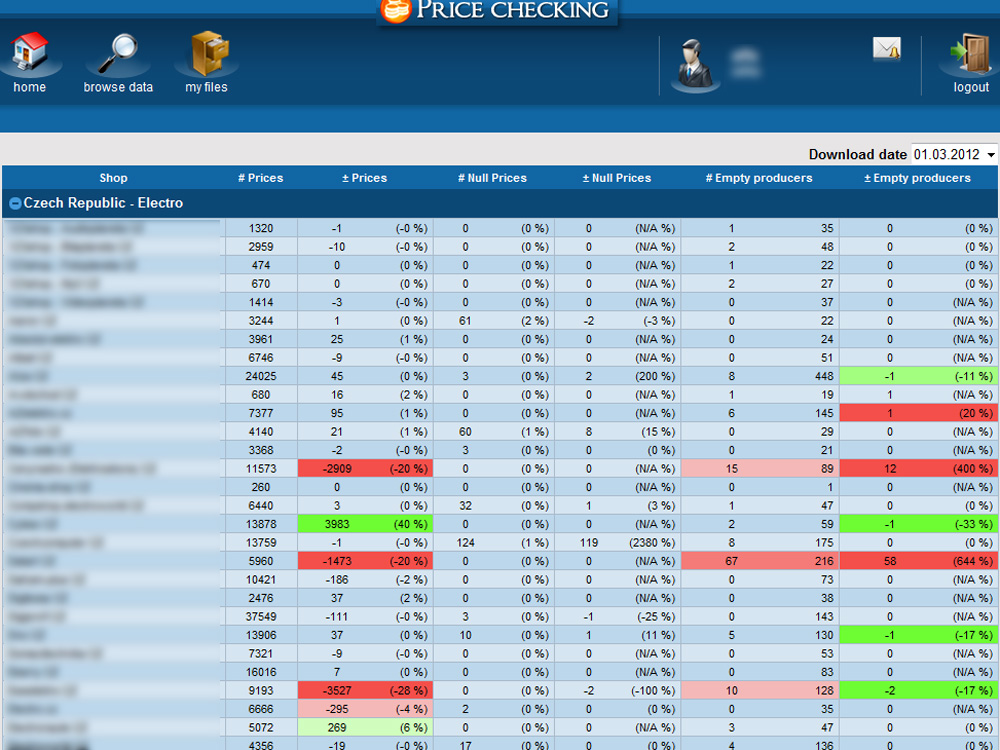
\includegraphics[width=0.9\textwidth]{resources/priceChecking}
	\caption[Price checking]{Ukázka služby Price checking}\label{fig:priceChecking}
\end{figure}

\newpage

\subsection{Pricing intelligence\cite{pricingIntelligence}} 

\textbf{Hlavní funkce}
\begin{itemize}
\item monitorování a srovnávání cen konkurence, vývoj cen a trendů v čase
\item přehledné výpisy výsledků
\item u většiny cenových nabídek nutno definovat počet konkurentů
\item upozornění na změny cen v čase
\end{itemize}

\textbf{Výstup}
\begin{itemize}
\item formát xsl nebo pdf
\end{itemize}

\textbf{Prostředí}
\begin{itemize}
\item webové rozhraní
\end{itemize}

\textbf{Data}
\begin{itemize}
\item nespecifikované data a zaměřený trh
\end{itemize}

\textbf{Cena}
\begin{itemize}
\item 599 až 4999 Kč měsíčně
\item minimálně tři měsíce
\item neomezené sledování produktů a konkurentů je možné pouze s nejvyšším tarifem a po individuální ceně
\end{itemize}


\subsection{Sledování trhu\cite{sledovaniTrhu}} 
\textbf{Hlavní funkce}
\begin{itemize}
\item sledování cen, pozic, dostupnosti a hodnocení na porovnávačích zboží i jednotlivých obchodech
\item uchování historie
\item možné napojení přímo na vlastní internetový obchod
\item notifikace změn
\item možnost více účtů s oddělenými přístupy
\item cenotvorba
\item detekce cenových spirál (kdo první zlevnil a následující dopady)
\end{itemize}

\textbf{Vstup}
\begin{itemize}
\item xml, xsl nebo manuálně
\end{itemize}

\textbf{Výstup}
\begin{itemize}
\item xsl nebo webový
\end{itemize}

\textbf{Prostředí}
\begin{itemize}
\item webové rozhraní
\end{itemize}

\textbf{Data}
\begin{itemize}
\item srovnávače cen: heureka.cz, zbozi.cz, najnakup.sk, pricemania.sk, ceneo.pl, nokaut.pl, argep.hu, preisroboter.de
\item přímé sledování na obchodu
\item z toho plyne záběr na český, slovenský, německý a maďarský trh
\item aktualizace až několikrát denně
\end{itemize}

\textbf{Cena}
\begin{itemize}
\item platba za každé vyhledání
\item individuální cena
\end{itemize}

\subsection{Pricebot \cite{priceBot}}

Web je datován roku 2015, avšak popis funkcí není dokončený. Obsahuje výplňový text, proto je popis funkcí nekompletní.

\textbf{Hlavní funkce}
\begin{itemize}
\item denní monitoring cen na heureka.cz
\item možnost sledovat produkty konkurence
\item poskytuje pravidelný výsledek nalezených cen a vizualizaci změn
\item notifikace o změnách
\item notifikace o konkurentech prodávajících za nižší cenu
\item maximum lze sledovat 600 produktů 
\item maximum sledovaných konkurentů je 70
\end{itemize}

\textbf{Vstup}
\begin{itemize}
\item produkty ke sledování
\end{itemize}

\textbf{Výstup}
\begin{itemize}
\item pdf na email
\end{itemize}

\textbf{Prostředí}
\begin{itemize}
\item webové rozhraní
\end{itemize}

\textbf{Data}
\begin{itemize}
\item srovnávač cen Heureka.cz
\end{itemize}

\textbf{Cena}
\begin{itemize}
\item dle počtů produktů
\item od 299 do 1299 Kč
\end{itemize}

\newpage

\subsection{Zahraniční nástroje}
Tyto nástroje jsou obecněji zaměřené a obvykle požadují od uživatele technické znalosti, 
jelikož je nutné přesně specifikovat kde, co a jak je požadováno sledovat. Vzhledem k tomuto omezení není možné
použití přímo provozovateli e-shopů, jelikož těmito znalostmi z povahy práce obvykle nedisponují.
\par
Příklad zahraničních nástrojů:

\begin{enumerate}
\item Screen scraper \cite{ScreenScraper}

  \begin{itemize}
    \item Webová služba
    \item procházení web skrz odkazy
    \item potvrzování formulářů
    \item využití interního vyhledávání
    \item export do širokého množství formátu souborů
    \item cena: \$549 - \$2,799 za měsíc
  \end{itemize}
  
\item Web extractor \cite{WebExtractor}

  \begin{itemize}
    \item Windows Aplikace
    \item procházení zadaných stránek
    \item hledání stránek pomocí klíčových slov
    \item export do csv formátu
    \item cena: \$99 - \$199 jednorázově
  \end{itemize}


\end{enumerate}

\newpage

\chapter{Analýza týmového projektu}
V této kapitole se budu věnovat řešení vytvořeného v rámci předmětů BI-SP1 a BI-SP2 na ČVUT FIT v akademickém roce 2015/16.
Popíšu cíl, který měl projekt za úkol řešit a jaká měla být výsledná funkcionalita řešení. Dále také vysvětlím základní strukturu
navrženého systému.

\section{Cíl týmového projektu}

V předmětech BI-SP1 a BI-SP2 byl realizován týmový projekt. V souladu s osnovami byl nejdříve v BI-SP1 vytvořen návrh
systému a v BI-SP2 následně implementován.
\par
Cílem tohoto projektu byla maximální možná míra automatizace získávání informací o produktech prodávaných konkurencí. Důraz byl především kladem na optimalizaci počtu nutných lidských úkonů. Byl navržen způsob, kdy systém při pouze nezbytných krocích spoléhá na administrátora.
U administrátora se předpokládá technická zdatnost průměrného uživatele.
\par

\section{Požadovaná funkcionalita}
Požadovaný stav projektu umožňuje uživateli vložit produkty do systému ve formátu \textit{cvs} či \textit{xlsx}, poté pomocí
rozhraní definovat význam jednotlivých sloupců v tomto dokumentu a zvolit požadovanou frekvenci sledování dat.
\par
Systém na základě dat vyhledá obchody, které prodávají sledované produkty. Z nich v definovaných intervalech získává data, ze kterých je vytvořen výstup pro uživatele obsahující především informace o cenách. Výstup lze vizualizovat i na grafech ve webovém rozhraní nebo stáhnout ve formátu
\textit{csv} či \textit{xlsx}.
\par
Proces samotného hledání byl navržen jako soubor více kroků, skládající se z procesů interních částí a interakcí administrátora, který zajišťuje
řešení problémů, které systém nedokáže vyřešit.

\section{Návrh}
Řešení bylo rozděleno na \textbf{část webového rozhraní} a na část zpracovávající interní procesy, nazývanou v této práci 
jako \textbf{interní část}.
Vzhledem k požadavkům na škálovatelnost aplikace se interní část skládá z více samostatných menších služeb - modulů komunikující
spolu pomocí front. Díky tomu, že každý modul zajišťuje určitou funkcionalitu a je možné vytvářet více jeho instancí. Procesy lze 
zpracovávat paralelně a na více serverech, kde je jediné kritérium připojení na systém zajišťující komunikaci.
\par
Uživatelská a interní část spolu sdílejí data pomocí relační databáze\cite{DB}.

\section{Webové rozhraní}

\subsection{Uživatelská část}\label{ch:analysis-front-end}
Uživatelská část obsahuje množinu podstránek určených pro koncové uživatele
služby(klienti).
\par
Uživatelská část umožňuje vytvořit kampaň. Kampaň je proces trvající určitý časový úsek, který sleduje vložené produkty na konkurenčních
obchodech.
V rámci běžící kampaně má poté uživatel možnost vidět vizualizaci získaných dat, případně je umožněn export dat do formátu
\textit{csv} či \textit{xlsx}. Ze zobrazených dat lze zjistit, na kterých webových stránkách je produkt prodáván a za jakou cenu.

\subsection{Část pro administrátory}
Pro přístup do části pro administrátory je nutné, aby měl uživatel speciální práva. Běžný uživatel, tak k této části nemá přístup. Slouží k monitorování kampaní uživatelů a řešení problémů, které systém není schopný 
automaticky vyřešit. Tím je myšleno definování selektorů pro výběr dat z webových stránek, párování produktu ke stránce 
nebo potvrzení zda jsou získaná data validní.

\section{Interní část}
Interní část je rozdělena do samostatných modulů, které spolu komunikují pomocí front. Moduly je možné spustit jako služby ve více 
instancích, kromě modulu Manager. Vzhledem k možnostem front, lze také práci distribuovat na více serverů, aniž by byla ohrožena 
bezpečnost databáze, protože k ní je možný přístup pouze lokální. Moduly jsou detailněji popsány v následujících podsekcích.
\subsection{Manager}
Manager je hlavní modul, který má jako jediný interní část možnost připojení do databáze a jeho běžící instance může existovat pouze jednou.
Manager má za úkol plánování práce pro ostatní části systému a samotnou správu komunikace s ostatními moduly. Práce je delegována pomocí
\textit{požadavků}, které jsou odeslány pomocí front jednotlivým modulům. \textit{Odpovědí} a \textit{chyby} reprezentují výsledky požadavků.
\subsection{Finder}
Modul Finder získává URL adresy internetových obchodů, které prodávají požadované produkty.
Na nalezeném obchodě poté vyhledává adresy vedoucí na detaily produktů. K tomu je použito interní vyhledávání, které
obchod poskytuje svým zákazníkům. Získané adresy detailů pak obsahují podrobné informace prodávaných produktů.

\subsection{DataProvider}
DataProvider je modul, který zpracovává adresy vedoucí na detaily produktů. Proces modulu reprezentuje následující seznam, kdy každý hlavní bod může skončit uvedenou chybou. Výsledek je odeslán ke zpracování Managerem.
\par
\begin{enumerate}
\item Stažení stránky
	\begin{itemize}
	\item Stažení selhalo
	\end{itemize}
\item Vyparsování dat pomocí šablony
	\begin{itemize}
	\item Šablona neexistuje nebo je chybná
	\end{itemize}
\item Analýza dat vůči historickým datům (pokud existují)
	\begin{itemize}
	\item Data jsou nevalidní
	\end{itemize}
\end{enumerate}



\chapter{Vývoj a implementace týmového projektu}
V této kapitole se věnuji průběhu vývoje týmového projektu a vytvořenému řešení. Popíši zvolené postupy při vývoji a 
jaké technologie byly vybrány.
\par
Poslední část rozebírá mou roli v tomto
projektu, protože téma bakalářské práce jsem měl již předběžně vybrané na začátku předmětu BI-SP2.

\section{Vývoj}
Vývoj byl rozdělen do 5 iterací, z nichž každá obsahovala 10 sprintů. 
V každé iteraci bylo definováno jakou musí obsahovat funkcionalitu, která bude na konci iterace prezentována vyučujícímu. Funkcionalita se skládala z jednotlivých úkolů rozložených do sprintů.
Úkoly byly přiděleny jednotlivým členům týmu. Stav úkolů uchovával systém Redmine\cite{Redmine}, který umožňoval sledovat jejich stav.
Úkoly bylo možné přiřadit k jednotlivým sprintům a iteracím, což umožňovalo přehled o plnění časového plánu.
\par
Jako verzovací systém byl zvolen systém Git, se vzdáleným repozitářem uložený na službě Gitlab \cite{gitlab}. Gitlab poskytuje webové rozhraní pro snadnou správu a spouštění služeb na základě definovaných aktivit v repozitáři. Repozitář se skládal ze 4 částí (větví):
\begin{itemize}
\item Master - hlavní větev uchovávající verze určené k nasazení na produkční server
\item Develop - vývojová větev obsahující aktuální stav vývoje
\item Feature - vedlejší větev vytvořená pro konkrétní úkol přidávající novou funkcionalitu
\item Fix - vedlejší větev určená pro úkoly opravující chybu
\end{itemize}
Protože přístup k modifikacím větví Master a Develop měl pouze vedoucí projektu, musel být pro každou Feature a Fix větev
vytvořen požadavek o zařazení(Merge request). Po kontrole vedoucím byl požadavek zařazen nebo vrácen k opravě.
\par
Na konci každé iterace byla poslední verze označená pomocí \textit{tagu} a poté prezentována vedoucímu.
Označení bylo zvoleno na základě pořadí iterace. 1. iterace je označena verzí \uv{0.1}.
\par
Pro vývoj se využil princip průběžné integrace. Každá verze byla zkompilována, otestována a zanalyzována na vzdáleném serveru.
Tyto činnosti zajišťovaly systémy Jenkins\cite{jenkins} a Gitlab. Po změně v repozitáři byl spuštěn úkol v Jenkins. Ten aplikaci sestavil, spustil testy a statickou analýzu kódu 
zajištěnou systémem SonarQube\cite{sonar}. Výsledky publikoval ve svém webovém rozhraní a zároveň v rozhraní Gitlab.  
\section{Implementace}


\subsection{Webové rozhraní}
Webové rozhraní je implementováno v jazyce PHP verze 7. Základem aplikace je aplikační rámec Nette\cite{nette}. Nette
obsahuje nástroje pro automatickou správu závislostí, komunikaci s databází, vytváření bezpečných formulářů, zabezpečení
aplikace, šablonovací systém a rozhraní pro tvorbu testů. 
\par
Nette je navrženo s myšlenkou použití MVC architektury, která odděluje
prezenční a logickou vrstvu. Zkratka MVC značí Model-View-Controller. V případě webového projektu v Nette představují vrstvu \textit{view} šablony.
Šablony definují vzhled webových stránek. \textit{Controller} vrstva se skládá z presenter tříd obsluhující šablony. \textit{Modelovou} vrstvu  zajišťují třídy servisní, vykonávající logické části aplikace jako 
například práci s \textit{repository} třídami nebo zpracování formuláře. \textit{Repository} se starají o přímou komunikaci s databází.

\begin{figure}[h]\centering
 	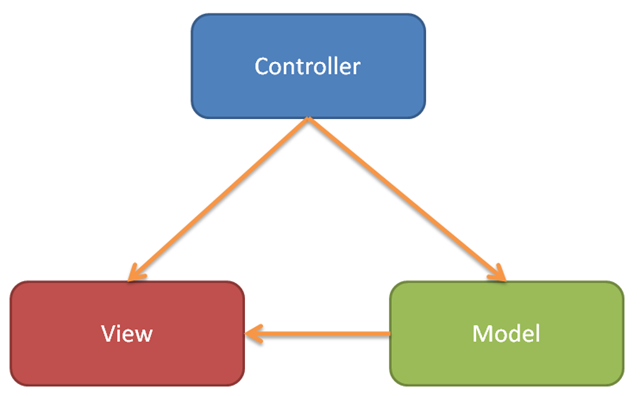
\includegraphics[width=0.7\textwidth]{resources/mvc}
	\caption[MVC]{Vizualizace návrhu MVC (Model-View-Controller}\label{fig:mvc}
\end{figure}
\par
Snadnou správu závislostí nad externími knihovnami zajišťuje balíčkovací systém Composer\cite{composer}. 
Na základě souboru definující potřebné knihovny a jejich verze jsou staženy z centrálního repozitáře. To zajišťuje jednotné verze
a eliminaci nutnosti knihovny manuálně stahovat či přidávat přímo do repozitáře.
\subsection{Interní část}
Interní část je implementována v jazyce Java verze 8. Sestavení, spouštění testů a správu závislostí zajišťuje Gradle\cite{gradle}.
Umožňuje automatické stažení knihoven. Standardně je nastavený jako zdroj
centrální maven repozitář. \cite{mavenRepo}. Maven repozitář uchovává většinu volně přístupných knihoven, v tomto případě všechny, které jsou v rámci tohoto projektu použity.
\par
V rámci sestavení lze pustit testy a další definované úkoly jako například tvorba dokumentace. Projekt používá
doplněk Cobertura\cite{cobertura}, který na základě spuštěné testovací sady vytváří zprávu obsahující pokrytí větví programu.
Díky tomu je možné jednoduše zjistit jaké větve aplikace nejsou otestované.
\par
Aplikace je rozdělena do nezávislých modulů běžící jako služby. Jednotlivé moduly spolu komunikují
pomocí posílání zpráv v definovaných frontách. Komunikaci zajišťuje systém RabbitMQ Server\cite{rabbitMQ} implementovaný v jazyce Erlang. Zprávy jsou serializovatelné objekty, jejichž definice je sdílena napříč všemi moduly.
\par
\textit{Serializace} představuje proces, kdy je objekt serializovaný do posloupnosti bitů, které jsou poslány jako zpráva. 
Vzhledem ke sdílené podobě objektu na obou stranách, lze zprávu jednoznačně deserializovat zpět do původního Java objektu se kterým
je možné dále pracovat.\cite{serialization}
\par
Projekt využívá mnoho volně dostupných knihoven, nejpodstatnější jsou však následující:
\begin{itemize}
\item Google Guice - automatická správa závislostí \cite{guice}
\item Hibernate - objektově relační zobrazení databázových entit a práce s nimi \cite{hibernate}
\item Apache Commons - pomocné knihovny pro práci s řetězcemi a soubory \cite{commons}
\item RabbitMQ - rozhraní pro komunikaci s frontami \cite{rabbitMQ}
\end{itemize}

\section{Má role}
V druhé části týmového projektu, samotné implementaci, jsem byl vedoucí týmu. Jelikož jsem již měl téma své bakalářské práce vybrané, 
věnoval jsem se projektu nad rámec předmětu. Kromě povinností vedoucího, které se skládaly z plánování práce a kontroly vytvořené implementace
jsem se věnoval návrhu, který bylo třeba v průběhu semestru pozměnit, jelikož návrh z předmětu BI-SP1 nebyl dostatečný. Jednalo například
o navržení modulu Manager, který byl navržen pouze jako black-box.
\par
Na začátku projektu jsem vytvořil celý ekosystém, tvořený z přidružených služeb použitých při vývoji.
Zde se jedná především o propojení následujících služeb s Gitlabem:

\begin{itemize}
\item Redmine - možnost prokliku na úkol na základě čísla ve zprávě verzované jednotky (commit message)
\item Jenkins - spouštění sestavení aplikace na základě nové verze, oddělené dle jednotlivých větví (hlavní, vývojová, vedlejší) a
				publikace výsledku
\item SonarQube - zobrazování interaktivního výsledku statické analýzy přímo v rozhraní Gitlab
\end{itemize}

Samotný SonarQube bylo potřeba nastavit, aby se spouštěl při sestavení aplikace a výsledek se zobrazil v rozhraní
Gitlabu. V rámci sestavení aplikace jsem nastavil spouštění nástroje Cobertura.
Doplňky v Jenkins umožňovaly zobrazení přehledných výsledků, jak je kód pokryt testy \ref{fig:cober-old}. Přesné pokrytí testů mi poté umožňovalo 
jednoduše kontrolovat jaké části kódu jsou otestované.


\chapter{Zhodnocení týmového projektu}
Pro návaznost na kapitolu o provedených vylepšeních je nejprve nutné uvést v jakém kontextu jsou navrhovány. K tomu je třeba
popsat výsledný stav projektu a jeho funkcionalitu, čemuž se budu věnovat v této kapitole.


\section{Stav}
Ačkoliv stav projektu odpovídal požadavkům na úspěšné odevzdání, nebyla dosažena implementace všech procesů. 
Tím bohužel nebylo možné reálné použití systému.
\par
Odevzdávaný stav obsahoval funkční webové rozhraní, které se skládalo ze základní funkcionality pro uživatele a administrátory.
Část pro administrátory obsahovala správu uživatelů, evidenci známých obchodů a řešení chyb vzniklých v interní části.
\par
Uživatelská část umožňovala správu a vytvoření kampaní. Splňovala návrh z analytické částí \ref{ch:analysis-front-end}.
Na žádost jiného týmu bylo také vytvořeno Web API rozhraní, poskytující získané ceny pro daný produktu ve formátu JSON.
\par
Interní část byla schopná pracovat pouze na základě dříve uložených url adres vedoucí na detaily produktů. 
Manager dokázal vybrat adresy detailů, které je potřeba aktualizovat.
\par
Na základě adres vytvořil Manager požadavky obsahující potřebná data. Požadavky odeslal pomocí front pro zpracování do DataProvideru. Ten na základě obdržených dat stránku stáhnul, vyparsoval a zanalyzoval výsledek vůči historickým datům a odeslal informace o produktu, který se na adrese nachází.
\par
Analýza se skládala z kontrol velkých výkyvů cen a rozdílných identifikátorů produktu.
V případě, že požadavek neobsahoval šablonu pro vyparsování nebo byl výsledek označen jako chybný, tato chyba byla odeslána zpět do Manageru, kde se  výsledek uložil pro zobrazení ve webovém rozhraní, ať už se jednalo o chybu
nebo nalezení ceny. Vyřešení chyby Manager detekoval a adresu využil k vytvoření nového požadavku.

\begin{figure}[h]\centering
 	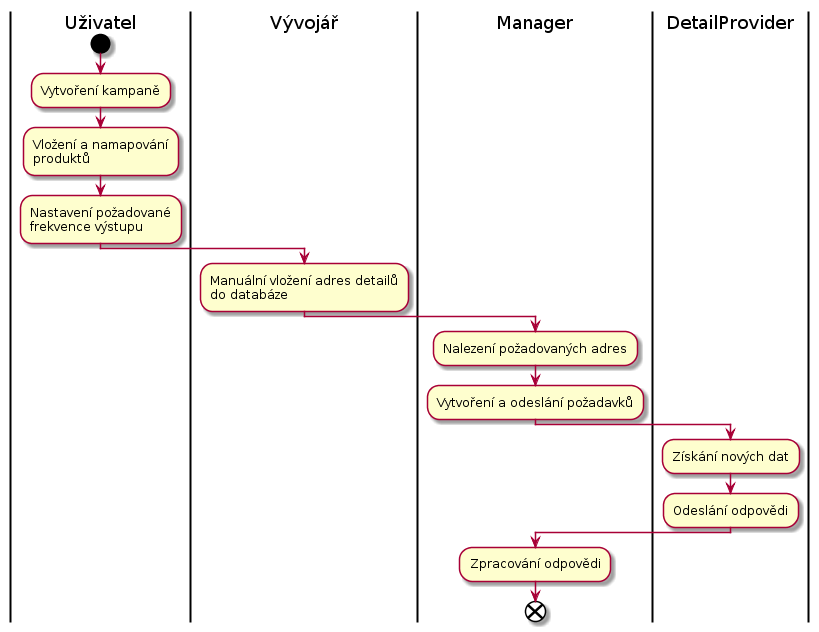
\includegraphics[width=1.0\textwidth]{resources/legacy-process-activity}
	\caption[Diagram zobrazující vytvoření kampaně a nalezení nových dat v původním řešení týmového projektu]
	{Diagram zobrazující vytvoření kampaně a nalezení nových dat v řešení týmového projektu.}\label{fig:legacyprocess-activity}
\end{figure}

\section{Nedostatky}
Vytvořené řešení obsahovalo spoustu nedostatků, které bylo třeba v rámci této práce detekovat a ty nejdůležitější se pokusit opravit.
Z důvodu kontextu a odlišnosti od původního návrhu nejprve popíšu systém plánování práce, který byl častý důvod nežádoucího chování systému.

\subsection{Vytváření požadavků pro ProductProvider}
Některé nedostatky byly úzce spjaty s tím, jak aplikace plánovala práci. Plánováním práce je myšlen proces
nalezení adres detailů produktů, kde je požadováno získat nové data. Z nich jsou vytvořeny požadavky pro ProductProvider k zpracování.
\par
Jak bylo řečeno, prvotním kritériem hledání jsou adresy detailů. Ty se mohou vyskytovat v různých stavech. Systém je vybral v 
následujícím pořadí:

\begin{itemize}
\item Adresy, které mají produkty v zaplacené kampani
\item Adresy bez produktů
\item Adresy, pro které neexistuje šablona pro parsování
\item Adresy, které mají vyřešenou chybu
\end{itemize}

Z této množiny bylo poté vybráno prvních 10 adres, odebrány již odeslané a ty které mají nevyřešenou chybu. Opakované spuštění v předdefinovaném 
intervalu zajistilo, že požadavky byly vytvořeny pro všechny požadované adresy.
\par
Další nedostatek se skládal z ukládání stavu do databáze. Část nejdůležitějších atributů vytvářeného požadavku byla uložena do databáze 
s příznakem odesláno. Tento příznak bylo nutné uchovávat i u chyb šablon nebo analyzátoru, kde je potřeba označit, že byly zpracovány. 
\par
V případě neúspěchu při odeslání požadavku už však příznak v případě chyb nebyl změněn. To způsobilo, že chyba nebyla v příštích hledání znovu zpracována.

\subsection{Neefektivní chování modulu Manager a ProductProvider}\label{ch:manager-pd}
První zásadní problém bylo neefektivní chování komunikace modulu Manager s ProductProviderem. V rámci testování jsem zjistil, že v 
případě chyby při parsování stránky není použit uložený HTML dokument.
To pramenilo z výše popsaného návrhu plánování, které nalezlo korektně adresy, ale vytváření samotného objektu představující požadavek,
bylo stejné pro všechny adresy. Vytváření neobsahovalo použití již staženého dokumentu, na jehož základě byla vytvořena 
chyba parsování nebo analyzování. Každý požadavek vyústil v opětovné stažení příslušné stránky.

\subsection{Chyby analyzování}
Poslední fáze procesu v modulu ProductProvider byla navržena jako analyzování získaných dat vůči již dříve uloženým. Implementace analyzátoru 
spouštěla jednotlivé validace, jejíchž logika se nacházela v oddělených třídách. 
Analýza kontrolovala zda se shoduje získaný EAN, název a modelové číslo, vůči uloženým identifikátorům. Pokud na jedné ze stran hodnota neexistovala, byly data označená, že jsou pravděpodobně chybná. Dále probíhala kontrola získané ceny \uv{s} a \uv{bez} DPH oproti cenám získaných na konkrétní stránce dříve.
\par
Kontrola porovnala průměr historických hodnot se získanými hodnotami cen. V případě, že rozdíl byl větší jak 25\%, byl výsledek označen jako
možná chyba.
\par
Pokud validační třída objevila nežádoucí data,
vyhodila výjimku, ve které byly uložené informace o chybě. Tento způsob řízení programu však způsoboval, že celá validace skončila při první chybě.
Zároveň obsah výjimky pouze určoval typ validace bez přídavných informací.
Informace byly následně odeslány a Manager na jejich základě vytvořil chybu pro administrátora k vyřešení. Administrátor tak mohl 
označit, zda je to opravdu chyba nebo se toto hlášení má do budoucna ignorovat.
\par
Problém nastával pokud se na adrese objevilo více chyb. To znamenalo, že každý požadavek vytvořil další
chybu analyzátoru a administrátor musel všechny vyřešit. Při každém požadavku pak bylo nutné obsah adresy znova stáhnout.

\subsection{Vytváření chyb šablon}
Jako další problém se ukázalo plánování práce založené na kritériu, kdy jsou k vytvoření požadavku vybrány všechny adresy, které neobsahují šablonu.
Myšlenka byla taková, že pro vytvoření samotné šablony, je nutné nejdříve stránku stáhnout, nechat vytvořit chybu parsování
a následně ji vyřešit.
\par
Systém však odeslal požadavek pro všechny uložené adresy na obchodě. To vyústilo ve vytvoření mnoha chyb, 
které musel administrátor postupně vyřešit.

\subsection{Modul Finder}
Modul Finder nebyl zapojený do systému. Existovala pouze hlavní implementace interních procesů, jejíchž funkčnost byla
pouze ověřena jednotkovými testy. Neexistující rozhraní pro práci s frontami a chybějící příslušné třídy Managera, které zajišťují vytváření příslušných požadavků neumožňovaly ověření celkové funkcionality této části. Z tohoto důvodu nebyl systém jako celek vhodný pro jakékoliv reálné použití, jelikož
jediná možnost jak využít funkcionalitu interní částí, bylo vytvořit SQL insert skripty, obsahující adresy detailů produktů
a ty spustit nad databází, kterou systém používal.
\par
Další důsledek byla neexistence procesu párování produktů. Finder byl navržený tak, že po nalezení internetového obchodu
pomocí interního vyhledávání nalezne detaily produktů, u kterých je velká pravděpodobnost, že patří hledanému produktu.
Zda se však jedná o správný detail produktu je však třeba ověřit, jelikož výstupem může být více adres. Po získání hodnot ze stránky se musí nežádoucí adresy vyloučit a ostatní spárovat s produktem.
\subsection{Plánování práce}
Projekt neobsahoval plánování práce vůči požadovanému intervalu, kdy mají být nová data
staženy. Aktuální stav hledal pouze adresy produktů, které se nachází v zaplacené kampani nebo měly vyřešenou chybu.
\subsection{Škálovatelnost}
Původní návrh počítal se škálovatelností aplikace na více serverech, kde je možné vytvořit neomezený počet instancí DataProvider a Finder. Reálný stav na konci projektu však tuto možnost neumožňoval. Interní část běžela jako jedna služba rozdělená do více modulů. 
Instance všech modulů probíhala v Managerovi, který musel mít přímou závislost na ostatních modulech.
\subsection{Obecný návrh a testy}\label{ch:architecture-tests}
Implementace samotná byla velmi nepřehledná. Vykytovaly se prvky značící špatný návrh aplikace.
Zde bych rád zmínil například dlouhé a nepřehledné metody v
DataProviderServiceImpl a AbstractFinderUrlListWorkerImpl, kde přestože jejich velikost 
nepřesahovala 60 řádků bylo velmi obtížné zjistit, co mají vykonávat. Problém byly také velké třídy
jako například DataProviderServiceImpl zajišťující celý proces v modulu DataProvider.
\par
Je nutné podotknout, že spousty špatných konstrukcí byla eliminována již v průběhu vývoje týmového projektu.
První důvod byla statická analýza kódu detekující konstrukce, které jsou zdrojem častých chyb. Statická analýza
však nebyla schopná najít všechny problémy. Druhý důvod byla moje kontrola při schvalování vytvořeného kódu pro 
zadaný úkol. Z důvodu časové tísně, ale nebyl vždy prostor na to vrátit kód k přepsaní a opravení všech nedostatků. To způsobilo, že
se vědomě dostaly do hlavních větví konstrukce, které nebyly považovány za ideální. Myšlenkou bylo, že budou přepracovány později, což se ne vždy povedlo.
\par
Další problém návrhu byly procesy v DataProvider modulu řízené pomocí výjimek obsahující 
přídavné informace. A to i v případech, kdy byl takový výsledek očekávaný nebo dokonce chtěný. 
Toto použití je však v rozporu ideou použití výjimek, které mají signalizovat neočekávaný stav, kdy není možné dále pokračovat.\cite{exception}
Pro uchování přídavných informací bylo nutné vytvářet výjimky vlastní, které obsahují přesnější údaje o chybě. Ani tyto údaje však nebyly 
dostatečné a tak nebylo možné přesně rozpoznat ve webovém rozhraní přesný důvod chyby.
\par
V kritických částech chyběly některé důležité testy, jelikož třídy snažící se dělat více věcí najednou, by bylo velmi
složité otestovat. Chybějící testy se vykytovaly například u následujících částí: databázová vrstva, fasády, vytváření požadavků pro DataProvider,
hlavní servisní třída DataProvideru nebo validace dat analyzátorem. Z tohoto důvodu jakákoliv oprava nebo implementace nových požadavků 
mohla narušit stávající funkcionalitu bez možnosti rychlého ověření. Tím by mohla být jakákoliv změna velmi časově náročná, s velmi nejistým konečným výsledkem.

Systém proto v tomto stavu nebyl vhodný pro následný rozvoj.

\begin{figure}[h]\centering
 	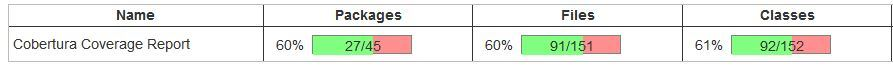
\includegraphics[width=1.0\textwidth]{resources/cobertura-report-old-1}
 	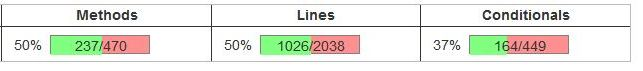
\includegraphics[width=0.7\textwidth]{resources/cobertura-report-old-2}
	\caption[Pokrytí testy vytvořeného řešení]{Pokrytí testy vytvořeného řešení. Získáno pomocí nástroje Cobertura. Vizualizace
	výsledků byla vytvořena při sestavení na Jenkins s příslušným doplňkem.}\label{fig:cober-old}
\end{figure}

\section{Shrnutí}\label{ch:project-analysis}
Jako metriky zhodnocení byly zvoleny následující kritéria seřazené od nejpodstatnějších k nejméně důležitým: 

\begin{itemize}
\item Kritické chyby
\item Úplnost požadované funkcionality
\item Rozšiřitelnost (návrh, pokrytí testy, statická analýza kódu)
\item Neefektivní chování
\item Uživatelská přívětivost
\item Škálovatelnost
\end{itemize}

Rozšiřitelnost je hodnocena na základě návrhu, pokrytí testy a počtu chyb statické analýzy kódu. Návrh byl podrobně zmíněn v kapitole 
\ref{ch:architecture-tests}. 

Na základě shrnutí nedostatků v tabulkách \ref{table:analysis-old1} a \ref{table:analysis-old2}je možné prohlásit, že pro základní použití systému je potřeba opravit kritické chyby a doplnění požadované funkcionality. Pro pohodlné použití je však zapracovat i na zbylých požadavcích, jinak je možné, že systém bude systém z hlediska administrátorského rozhraní velmi nepřívětivý. Neefektivní chování se může negativně odrazit při velké zátěži. Škálovatelnost má v tomto případě prioritu nejmenší.

\begin{table}[h]\centering\label{table:analysis-old1}
	\caption[První část tabulky přehledu nedostatků vytvořeného týmového řešení]{První část tabulky přehledu nedostatků vytvořeného týmového řešení}
    \begin{tabular}{ | l | l | p{7cm} |}
    \hline
    Typ & Počet & Popis \\ \hline
    Kritické chyby & 2 &
    	\begin{itemize}
  			\item V případě chybného odeslání není chyba šablony nebo analyzátoru znova zpracována.
  		\end{itemize}\\ \hline
	\hline
    Úplnost funkcionality & 4 & 
    	\begin{itemize}
  			\item Systém nevyhledává internetové obchody.
  			\item Systém nevyhledává adresy detailů produktů.
  			\item Systém neplánuje práci v požadovaných intervalech.
  			\item Neexistence procesu párování.
  		\end{itemize} \\ \hline
	\hline
	Rozšiřitelnost &  & 
		\begin{itemize}
  			\item Návrh tříd byl vyhodnocen jako nevhodný pro rozšiřování.
  			\item Pokrytí testy dle nástroje cobertura. - 60\%.
  			\item 3 kritické chyby statické analýzy kódu.
  			\item 1 minoritní chyba statické analýzy kódu.
  		\end{itemize} \\ \hline
    \end{tabular}
\end{table}
\begin{table}[h]\centering\label{table:analysis-old2}
	\caption[Druhá část tabulky přehledu nedostatků vytvořeného týmového řešení]{Druhá část tabulky přehledu nedostatků vytvořeného týmového řešení}
    \begin{tabular}{ | l | l | p{7cm} |}  
    \hline
    Typ & Počet & Popis \\ \hline
	Neefektivní chování & 4 & 
		\begin{itemize}
  			\item Stránka je nově stažena v každém požadavku (i v případě chyby).
  			\item V případě chybného odeslání není chyba šablony nebo analyzátoru znova zpracována.
  			\item Každá chyba analyzátoru znamená samostatný požadavek a chybu.
  			\item Vytvoření více požadavků pokud neexistuje šablona na obchodě.
  		\end{itemize} \\ \hline	
	\hline
	Uživatelská přívětivost & 2 & 
		\begin{itemize}
  			\item Nutnost řešit chyby analyzátoru po jedné.
  			\item Řešené chyby neobsahují bližší informace (informace o chybě, vyparsované hodnoty, použitá adresa detailu).
  		\end{itemize} \\ \hline	
	\hline
	Škálovatelnost & 1 & 
		\begin{itemize}
  			\item Nemožnost vytvořit více instancí modulů.
  		\end{itemize} \\ \hline
    \end{tabular}
\end{table}


\chapter{Návrhy na vylepšení}
V této kapitole se věnuji návrhům na možná vylepšení. Samotné implementaci se poté věnuji v následující kapitole. 
Nedostatky, které byly zjištěny až v průběhu implementace vylepšení a nebyly zároveň i opraveny, budou zmíněny v kapitole týkající se zhodnocení
provedených vylepšení.

\section{Refaktorování stávajícího řešení}
Problémy původního řešení je třeba opravit. Na existujícím kódu však není možné stavět opravy nebo přidání nových funkcionalit. Příčinou jsou konstrukce jako zneužívání výjimek, dlouhé metody, velké třídy nebo dlouhé seznamy parametrů.
Z těchto důvodů je třeba vhodně interní část refaktorovat tak, aby bylo možné kód lépe udržovat a rozvíjet. Provedené změny následně 
otestovat pomocí jednotkových testů.
\par
V rámci refaktorování je nutné se pokusit zachovat co nejvíce původního kódu, obzvlášť takového, kde je ověřena funkcionalita.
Dále pro větší přehlednost přesunout všechny servisní třídy do samostatného balíku a sjednotit je. Jednotlivé funkcionality
budou poté v samostatných balíčcích.
\par
Při úpravách týkající se rozdělování jednotlivých tříd, musí být dán důraz na jejich přehledné a rozšiřitelné komunikační rozhraní.

\subsection{Řízení aplikace}
Chování modulu ProductProvider je řízeno pomocí chytání výjimek obsahující informace o chybě. 
Výjimky by bylo vhodné odstranit a návratové hodnoty změnit na objekt obalující celkový výsledek. Tento návrh poté ulehčí běh procesů, kde není žádoucí
skončit při první chybě. Kód bude možné lépe rozdělit a metody následně zkrátit, což výrazně zlepší přehlednost kódu.

\section{Plánování práce}
Samotná logika plánování práce, nebo-li nalezení adres detailů produktů, které chceme použít při vytváření požadavků, se ukázala být nedostatečná. Chybí požadovaná funkcionalita, tedy použití intervalu určující, kdy je požadován nový výstup. Není také implementováno odstranění adres u kterého není vyžadováno vytvářet a odesílat nový požadavek.
\par
Nový návrh hledá adresy podle těchto kritérií:

\begin{itemize}
\item Adresy, které mají produkty v aktivní kampani a požadovaný interval hledání odpovídá aktuálnímu dni
\item Adresy bez produktů
\item Adresy, pro které neexistuje šablona pro parsování
\item Adresy, které mají vyřešenou chybu
\end{itemize}

Po nalezení těchto disjunktních množin a odstranění duplicit jsou vyřazeny adresy, které z nějakého důvodu nevyhovují svým stavem.
Nežádoucí stavy jsou momentálně tyto:

\begin{itemize}
\item Pro obchod existuje nevyřešená parsovací chyba
\item Existuje nevyřešená chyba analyzátoru
\item Požadavek pro adresu byl již odeslán
\end{itemize}

Z důvodu možnosti, že nežádoucí stavy bude pravděpodobně požadované přidat či odebrat, je potřeba implementaci navrhnout tak, aby bylo možné kontroly kdykoliv modifikovat bez velkých zásahů do interní funkcionality.

\section{Oprava komunikace Manager - ProductProvider}
Vzhledem k problémům popsaných v kapitole \ref{ch:manager-pd} je požadováno komunikaci modulů Manager a ProductProvider optimalizovat.
Neefektivní chování by se mohl ukázat jako velký problém při zpracování velkého počtu dat, z důvodu nutnosti opakovaného
stahování webových stránek. 
\par
Při analýze kódu se ukázalo, že v aktuálním návrhu aplikace není možné tuto funkcionalitu jednoduše implementovat, aniž by se nejednalo o rychlou opravu neefektivním řešením. Oprava by znamenala, že pro každou vytvářenou adresu se systém musí pokusit najít
existující chybu a následně využít staženou stránku. Hledání by tak probíhalo ve většině případů zbytečně, jelikož chyba by neexistovala.
\par
Korektní oprava je úzce spjata s předchozími kapitolami, především s refaktorováním a úpravou plánování práce. Pokud úprava plánování zachová
informaci o přičině udávající, proč je adresa pro vytvoření požadavku zařazena, stačí poté pouze nalézt potřebné atributy a ty uložit.
\par
Informace by však měla být zachována i při odesílání, kdy se nastaví i příznaky o odeslání a zpracování šablony. V případě
kdy se požadavek nepodaří odeslat musí příznak odpovídat tomuto stavu. Z hlediska DataProvider stačí pouze zkontrolovat, zda existuje
stažená stránka v požadavku a v kladném případě ji nestahovat znova.

\section{Spojení chyb analyzátoru a vylepšení rozhraní} \label{analyser-join}
Analyzátor provádí kontrolu získaných dat. V případě podezření o nevalidních datech je vytvořena chyba určená k vyřešení
administrátorem. Validace kontrolují ekvivalenci identifikátorů vůči již uloženým a velké výkyvy cen na daném obchodu.
\par
Administrátor má možnost chybu vyřešit a uložit příznak, aby se chyba do budoucna ignorovala. Toto rozhodnutí je však
založené pouze na informaci obsahující jaká validace se nepovedla. Nemá možnost porovnat jaká data byla využita při validaci.
Webové rozhraní aktuálně nemůže možnost zobrazit dodatečná data, protože nejsou k dispozici. Interní část by měla takové informace
získávat a uložit do databáze. Následně může webové rozhraní tyto informace použít.
\par
V případě adresy, která obsahuje více chyb, je nutné řešit každou samostatně. Po každém vyřešení se musí počkat na zpracování interní částí.
Pro zrychlení je tak nutné požadováno chyby spojit do jedné, tak aby administrátor mohl vyřešit všechny možné chyby analyzátoru najednou.

\section{Monitorování}
Na virtuálním serveru probíhá sestavení aplikace, včetně všech dodatečných procesů. Zároveň zde běží vývojová a produkční verze interní i webové části.
Momentální stav poskytuje pouze omezenou možnost, jak sledovat využití prostředků virtuálního serveru.
\par
Pro lepší přehled běžících prostředků by bylo tedy vhodné zvolit monitorovací službu, která umožňuje unifikovat sledování
probíhajících procesů na serveru, včetně vytížení a zobrazuje stav na jedné stránce.

\section{Získání adres obchodů a příslušných detailů produktů}
Interní část vyžaduje ke své funkcionalitě již uložené adresy detailů produktů, ze kterých jsou získávána data pro produkty.
Původní návrh počítal s modulem Finder, který se bohužel nepodařilo zapojit v rámci týmového projektu. Ten 
měl za úkol hledat internetové obchody na cenových srovnávačích a na nich pomocí vyhledávaní nalézt konkrétní adresy.
\par
Funkce Finderu je navržena jako duální, zajišťuje jak hledání samotných obchodů, tak i detailů adres. Komunikační třída představující příslušný požadavek, proto musí obsahovat příznak o jaký typ požadavků se jedná. Jelikož předávané informace
jsou odlišné, vytvořený požadavek obsahuje velké množství prázdných hodnot, což přispívá k celkové nepřehlednosti.
\par
Z tohoto důvodu navrhuji rozdělení Finderu na dva samostatné moduly. První bude zastávat funkci hledání obchodů a druhý
vyhledávat na obchodu a získávat požadované adresy detailů produktů na daném obchodě.


\section{Párování produktu}
Po nalezení adresy detailu produktu, stažení v DataProvider modulu a následném vyparsování hodnot je třeba adresu spárovat s 
produktem uloženým v databázi. Příčinou nutnosti párování je, že po nalezení adresy detailu není jisté, jestli opravdu patří produktu, pro který 
byla nalezena. 
\par
Párování musí být provedeno s velkou jistotou. Z tohoto důvodu navrhuji vytvořit proces, který se nejprve pokusí produkt spárovat na základě
přesné shody některého z identifikátoru, což představuje název, modelové číslo nebo EAN produktu. 
\par
Proces není možné zcela zautomatizovat, jelikož část internetových obchodů nemusí poskytovat informace totožné s těmi uloženými.
Obchod může používat odlišný název. Odlišnosti identifikátorů může způsobit například jiná barva nebo přidaná velikost za nebo před modelové
číslo. Jako řešení se jeví hledat podřetězec modelového čísla a EANu, což řeší i problém pokud je ze stránky vyparsován text okolo
identifikátoru. Obchod také může poskytovat pouze název. To lze demonstrovat na obchodu \textit{glamot.cz}, například
pro produkt 
\href{https://www.glamot.cz/p/19128/difuzer-k-vysouseci-babyliss-pro-difuser-murano}{BaByliss PRO Difuser Murano \textit{[cit. 24.4.2017]}}.
\par
V případě neúspěchu párování, musí existovat možnost produkt spárovat manuálně, tedy akcí administrátora. 
Výše uvedený proces poté spoléhá na to, že vložená data při vytváření kampaně jsou validní. V případě nevalidních dat utřeba
příliš obecných a krátkých názvů, by párování proběhlo chybně.


\section{Neimplementované návrhy}
\subsection{Pokročilé párování produktu}
Párování produktu lze vylepšit o uchovávaní více hodnot pro identifikátory produktů, které systém může použít při dalším 
párování na jiných obchodech. Ukládání nových identifikátorů by mělo probíhat pouze se souhlasem administrátora tak, aby byla zajištěna validita dat.

\subsection{Uchování a využití hodnot z nespárovaných adres}
Vyhledáváním na obchodu je zpravidla výsledek, který obsahuje více adres detailů produktu. Většina jich je v době hledání nepotřebná, nicméně v budoucnu by mohly být využity. 
Pro dlouhodobě efektivnější chod systému se jeví praktické uchovávat získaná data z těchto detailů.
V případě přidání nových produktů do systému se poté pokusit najít shodu v těchto datech. To umožní odlehčení zátěže
na stahování stránek a celkově zrychlí chod systému.
\par
Adresy však mohou být neaktuální. Zde je proto nutné nastavit mechanismus ověření funkčnosti adres detailů produktů.


\chapter{Realizace vylepšení}
Kapitola realizace vylepšení se věnuje implementovaným vylepšením. Popisuje jak byly navržené změny provedeny.
V průběhu realizace byly objeveny nové nedostatky, z nichž některé byly také zpracovány, i když se s nimi původně nepočítalo.
Změny jsou v repozitáři webového rozhraní a interní části označeny. Původní verze týmového projektu byla označena jako
tag \textit{v0.53}, realizované vylepšení jsou poté označeny jako \textit{v0.6}

\section{Refaktorování stávajícího řešení}
První krok realizace bylo refaktorování stávajícího řešení. Zde bylo provedeno především přesunutí tříd do jednotného balíčku, 
rozdělení tříd, zkrácení metod, zmenšení počtu parametrů metod a nahrazení výjimek za návratové typy.

\subsection{Servisní třídy}
Pro větší přehlednost byly všechny servisní třídy přesunuty do nadřazeném balíčku \textit{service}. 
Servisní třídy jsou takové, které nespadají do ani jedné z těchto skupin:

\begin{itemize}
\item Obsluha frekvenčního probouzení aplikace v daném intervalu
\item Rozhraní komunikující s frontami
\item Třídy přistupující k databázi (DAO)
\item Fasády, které obalují komunikaci servisních a DAO tříd
\item Konfigurační soubory automatické správy závislostí
\item Komunikační třídy
\item Pomocné třídy
\end{itemize}

Třídy jsem pojmenoval pomocí nové konvence, kdy důležité servisní třídy obsahují prefix jakého modulu se týkají
a postfix \textit{service}. Důvodem byla větší přehlednost v projektu, kdy docházelo k podobným názvům napříč moduly.
\par
Změnu lze demonstrovat například na třídě zajišťující získávání dat ze stažené stránky. Třída \textit{cvut.fit.dataprovider.parser.ParserImpl} byla pak změněna na \textit{cvut.fit.dataprovider.service.parser.DPParserServiceImpl}. Uvedené názevy jsou včetně 
nadřazených balíčků, kdy například název třídy je v prvním případě pouze \textit{ParserImpl}.

\subsection{Řízení aplikace}
Aplikace, především v DataProvider modulu byla řízena pomocí výjimek, které způsobovaly problémy v návrhu a samotné funkcionalitě.
V návaznosti na návrh byly nahrazeny úpravou návratového typu, který obsahuje příznak výsledku 
a další příslušné informace.
\par
Návratový typ lze demonstrovat na následují zkrácené třídě \textit{DPParserRespose}, která je vrácena v DataProvider modulu
po provedení parsování.

\begin{lstlisting}[language=Java]
/**
 * Entity to keep parsed response. Almost every 
 * attribute can be null, 
 * so getters return {@link Optional} of nullable type.
 *
 * @author Jakub Tucek
 * @created 24.1.2017
 */
public class DPParserResponse {

    /**
     * Flag for keeping result of parsing
     */
    boolean finishedProperly;

    /**
     * Parsed name of the product
     */
    private String name;

    public boolean isFinishedProperly() {
        return finishedProperly;
    }

    public void setFinishedProperly(
    	boolean finishedProperly) {
    	
        this.finishedProperly = finishedProperly;
    }

    public Optional<String> getName() {
        return Optional.ofNullable(name);
    }

    public void setName(String name) {
        this.name = name;
    }
}
\end{lstlisting}

Tato struktura je použita jako návratový typ rozhraní a implementace části pro parsování hodnot 
ze stažené stránky v modulu DataProvider. Ukazuje použití příznaku označující, zda parsování proběhlo korektně. Další důležitý prvek
je zapouzdření proměnných uchovávající data.\cite{encapsulation} Přístup k proměnným je umožněn pouze pomocí \textit{get} a \textit{set} metod.
\par
Metody \textit{get} jsou oproti standardnímu návrhu pozměněny a nevrací přímo proměnnou, ale \textit{Optional} této proměnné.
Optional je kontejner, který může obsahovat požadovanou hodnotu \cite{optional} nebo být prázdný. Před přístupem k hodnotě je proto vyžadováno se objektu zeptat na jeho stav. Očividnost prázdnoty návratové hodnoty nutí vývojáře s touto možností počítat, čímž 
je omezen výskyt nežádoucích výjimek, především \textit{NullPointerException} \cite{nullPointerException}.
\par
Po nahrazení návratovými typy, jsou výjimky použity pouze v případech, kdy nastal neočekávaný stav a je nutné přerušit následující akce.

\subsection{Odstranění výjimky a spouštění validací}
Odstranění výjimek z interní části lze demonstrovat na změnách tříd zajišťující analyzování získaných výsledků v modulu DataProvider. Hlavní změny v této části jsou tři.
\par
První je přesunutí hlavního rozhraní \textit{Analyser} a jeho implementace
\textit{AnalyserImpl} z balíčku \textit{cvut.fit.dataprovider.analyser} 
do  \\
\textit{cvut.fit.dataprovider.service.analyser}. 
\par
Druhá změna představuje změnu rozhraní, kdy bylo potřeba
zmenšit počet parametrů a odstranit výjimku, která byla vyhozena v případě nalezení chyby. 
\par
Třetí změnou je samotné spouštění validací. V původním řešení byla třída závislá na všech příslušných validacích, které spustila.
Skončila však vždy při první chybě, což je jedna 
z příčin chování, které jsem popsal v kapitole poukazující na možnosti spojení chyb analyzátoru \autoref{analyser-join}.
\par
Vytvořil jsem nový návrh, který je použit i na ostatních místech interní části v závislosti na
prováděných vylepšeních. Analyzující servisní třídě jsem odebral jednotlivé závislosti na konkrétních validacích a nahradil je množinou 
obsahující validační rozhraní. Validační rozhraní je nastaveno v konfiguračním souboru automatické správy závislostí, kde je možné
definovat jaké validace se mají použít.
\par
Validačnímu rozhraní byl změněn návratový typ na \textit{Optional} třídy obsahující zprávu o chybě. Pokud chyba nenastala, je vrácena
prázdná hodnota. Implementace těchto rozhraní byly rozděleny podle toho, jakou hodnotu kontrolují.
Při úpravě validací jsem zároveň zjistil, že základní validace lze rozdělit na dvě skupiny: validace řetězce a čísla.
\par
V případě těchto skupin se vytvořený kód lišil pouze v tom, jaká hodnota se má získat ze získaných dat a z dat již uložených.
Poslední rozdíl byl pouze v chybové hlášce. Z toho důvodu jsem společnou logiku obou skupin implementoval
pomocí abstraktní a generické třídy \textit{AbstractAnalysis}. Vlastnosti kontrol jednotlivých skupin zajišťují třídy \textit{AbstractStringAnalysis} 
nebo \textit{AbstractPriceAnalysis}. Výsledná validace kontroluje, zda získaná hodnota odpovídá již uložené hodnotě, vypadá následovně:

\begin{lstlisting}[language=Java, caption={Validace kontrolující hodnotu získaného jména produktu}]
/**
 * NameAnalysis is extension of {@link AbstractStringAnalysis} for analysing Name.
 *
 * @author Jakub Tucek
 * @created 27.1.2017
 */
public class NameAnalysis extends AbstractStringAnalysis {

    /**
     * {@inheritDoc}
     */
    @Override
    boolean skipAnalysis(DataProviderRequest request) {
        Optional<ComAnalyserFlags> analyserFlags = request.getAnalyserFlags();
        return analyserFlags.map(ComAnalyserFlags::isIgnoreDifferentName)
                .orElse(false);
    }

    /**
     * {@inheritDoc}
     */
    @Override
    Optional<String> getOptionalProperty(DPParserResponse parserResponse) {
        return parserResponse.getName();
    }

    /**
     * {@inheritDoc}
     */
    @Override
    List<String> getComProductValues(ComProduct comProduct) {
        return comProduct.getNames();
    }

    /**
     * {@inheritDoc}
     */
    @Override
    AnalysisErrorMessage generateAnalysisErrorMessage(String comProductValue, String parsedValue) {
        return new AnalysisErrorMessage()
                .withErrorMessage(
                        String.format("Parsed name value[%s] doesn't match known name value[%s]",
                                parsedValue, comProductValue)
                )
                .withErrorType(AnalysisErrorType.DIFFERENT_NAME);
    }
}
\end{lstlisting}
Jednotlivé validace implementují pouze metody, které vrací jaká hodnota byla získaná a historické hodnoty. Dále kontroluje zda
danou validaci ignorovat či nikoliv. Poslední implementovaná metoda vytváří informace o případné chybě. Tuto informaci je poté
možné využít v zobrazení administračním rozhraní. V původním řešení tato možnost chyběla, administrátor musel o chybě rozhodnout pouze
na základě typu chyby a adresy vedoucí na detail produktu. K tomuto vylepšení se vracím v samostatné kapitole.
\par
Konečné spuštění validací bylo ve výsledku zkráceno na metodu obsahující jeden řádek kódu, ačkoliv tento řádek
obsahuje více zřetězených volání.
\par
\begin{lstlisting}[language=Java, caption={Upravená implementace hlavní metody ve třídě zajišťující spouštění validací analyzátoru}]
    /**
     * Runs analysis for given {@link DataProviderRequest} and {@link DPParserResponse}.
     * Error are returned as list of {@link AnalysisErrorMessage}.
     * Injected set of {@link Analysis} is executed one by one, result unwrapped and kept if present.
     * Set of analysis result error messages is returned.
     *
     * @param request        dp request
     * @param parserResponse parsed data
     * @return list of errors or empty (if result was valid)
     */
    @Override
    public List<AnalysisErrorMessage> runAnalysis(DataProviderRequest request, DPParserResponse parserResponse) {
        return analysisSet.stream()
                .map(x -> x.analyse(request, parserResponse))
                .filter(Optional::isPresent)
                .map(Optional::get)
                .collect(Collectors.toList());

    }
\end{lstlisting}
\par
\begin{lstlisting}[language=Java, caption={Původní implementace hlavní metody ve třídě zajišťující spouštění validací analyzátoru}]
    /**
     * Analyses the new product info in comparison with the history
     *
     * @param newInfo        the new product info to be analysed
     * @param newData
     * @param oldInfo        the old product info
     * @param productHistory the history of the product info   @throws AnalyserException when analysing fails, contains error type
     * @param analyserFlags
     */
    @Override
    public void analyse(ComProduct newInfo,
                        ComProductHistory newData,
                        ComProduct oldInfo,
                        List<ComProductHistory> productHistory,
                        ComAnalyserFlags analyserFlags) throws AnalyserException {
        ValidatorData data = new ValidatorData(newInfo, newData, oldInfo, productHistory, analyserFlags);
        try {
            eanValidator.validate(data);
            partNumberValidator.validate(data);
            priceValidator.validate(data);
            namesValidator.validate(data);
        } catch (AnalyserException e) {
            logger.info("Analysis failed for product id: {}", newInfo.getProductId(), e);
            throw e;
        }
        if (!data.getWarnings().isEmpty()) {
            //No handling neeeded at the moment
        }
    }
\end{lstlisting}

\begin{figure}\centering
 	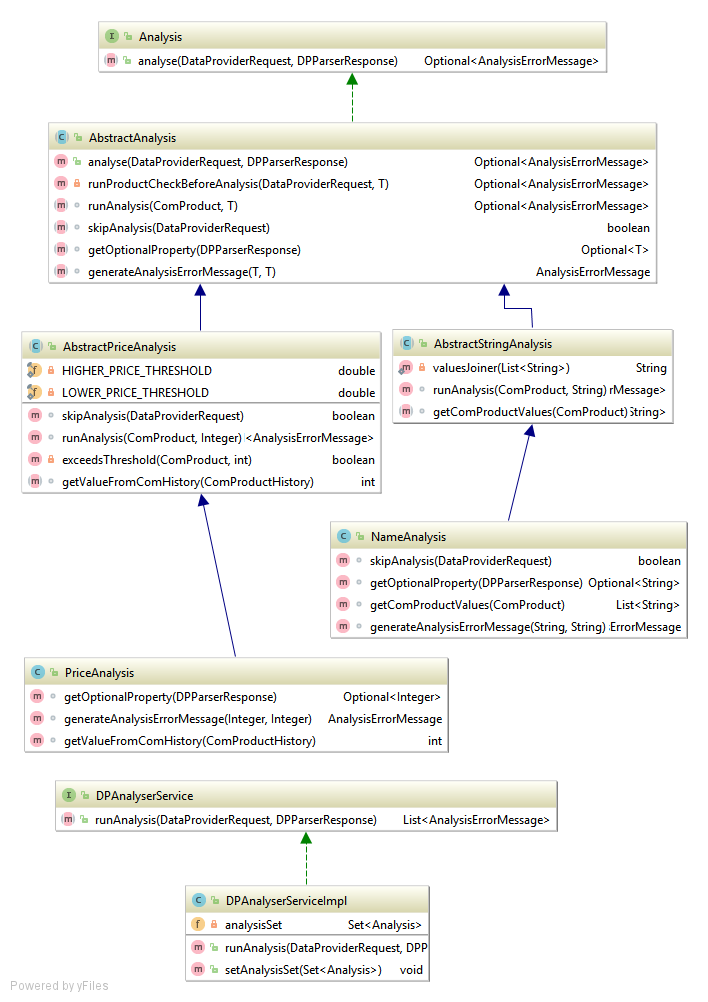
\includegraphics[width=1.0\textwidth]{resources/analyser-classes}
	\caption[Diagram tříd analyzátoru]{Diagram tříd analyzátoru. Obsahuje pouze některé validace z důvodu přehlednosti.}\label{fig:analyser-classes}
\end{figure}


Jak již bylo zmíněno, podobná architektura spouštění validací se vyskytuje na více místech interní části, například validace po provedení
parsování nebo kontrol, zda má být požadavek či adresa použita při plánování práce.


\section{Plánování práce}\label{ch:planning}
Plánování práce bylo rozděleno do tří částí, Nalezení adres, vytvoření požadavků a samotné odeslání.
Tato kapitola se týká pouze samotného nalezení adres, které je požadováno použít v dalším zpracování.
\par
V rámci hledání samotných adres byly implementovány servisní třídy, které samotné adresy hledají podle kritérií popsaných v 
návrhu vylepšeních. Následně jsou vráceny rozdělené dle způsobu nalezení. Nalezení adres nově počítá i s frekvencí, 
která je nastavena u aktivní kampaně.
\par
Nalezené adresy všech typů jsou vyfiltrovány o nežádoucí stavy. K tomuto účelu jsem navrhl rozhraní kontrol, rozhodující 
o tom, zda adresu použít. Tento návrh se podobá validačním kontrolám analyzátoru v modulu DataProvider.

\section{Oprava komunikace Manager - ProductProvider}
Důležitý prvek samotné opravy komunikace modulů Manager a ProductProvider je vytváření požadavků z nalezených adres.
Vzhledem k změně rozhraní, které zachovává způsob nalezení, stačilo vytvořit ostatní části Managera, tak aby odpovídalo novému rozhraní.
\par
Hlavní metoda servisní třídy \textit{DPRequestSenderServiceImpl} volající všechny tří části vypadá následovně:
\begin{lstlisting}[language=Java]
    /**
     * Creates requests and sends them.
     *
     * @throws MQConnectionException when sending fails
     */
    @Override
    public void createRequests() throws MQConnectionException {
        ProductUrlSets requiredProductUrls = prioritizeService.findRequiredProductUrls();

        DPRequestProductUrlWrapper dpRequestWrapper = requestBuilderService.create(
                requiredProductUrls);


        senderService.sendDPRequests(dpRequestWrapper);
    }
\end{lstlisting}
Nejdříve jsou nalezeny adresy, což bylo popsáno v kapitole \ref{ch:planning}. Po nalezení jsou vytvořeny výsledné požadavky
a odeslány. Servisní třída zodpovědná za odeslání zároveň ukládá příznaky stavu do databáze.
\par
Vzhledem v zásadní změně architektury neuvádím původní kód, jelikož celkový způsob vytváření požadavků je značně odlišný a není proto možné jednoduché porovnání. Vytváření bylo v předchozím řešení ve stejné třídě, která zajišťovala i odesílání, což způsobovalo problém při ukládání příznaků do databáze.
\par
Nový návrh vytváření požadavků tento proces deleguje do nové 
třídy  \\ \textit{DPRequestBuilderServiceImpl}, která zajišťuje uložení všech potřebných atributů do nového požadavku. Návratový typ této třídy slučuje množiny požadavků obsahující adresy bez produktů a 
ty v aktivní kampani, jelikož po vytvoření požadavků není potřeba odlišné chování k těmto požadavkům. Ostatní množiny jsou 
zachovány. Vzhledem k potřebě pracovat s adresou detailu i při odesílání požadavků, obsahuje \textit{DPRequestProductUrlWrapper}
množiny obsahující dvojice požadavku a adresy detailu. Důvod je odpadnutí nutnosti hledání chyby podle identifikátoru, což je potřeba
při ukládání příznaku chyby o zpracování.

\subsection{Odesílání požadavků}
Odesílání požadavků jsem upravil, aby odpovídalo novému návrhu. Před odesláním je každý požadavek uložen do databáze a nastaven
příznak o zpracování. V případě neočekávané chyby při odesílání, jsou tyto příznaky korektně změněny.
\par
Samotné odeslání má u všech požadavků stejný postup. Nejprve jsem proto extrahoval části obsahující ukládání a změnu stavu požadavků či chyb do samostatné třídy
\textit{DPRequestPersistServiceImpl}. Poté jsem využil nativního rozhraní Java 8 \textit{Consumer<T>}, které reprezentuje
operaci, která přijímá jeden vstup a nevrací žádný výsledek. Rozhraní jsem použil k reprezentaci operace uložení a
změny stavu v případě chyby.
\par
\begin{lstlisting}[language=Java, caption={Společná metoda zajišťující odeslání DataProvider požadavků}]
    /**
     * Sends request via {@link RequestHandler}.
     * Request is first persisted via {@link PersistanceDPRequestFacade} and it's id is set to the request in wrapper
     * object. If failure while sending object through MQ occurs, then {@link Consumer} failureHandler is called,
     * exception logged and rethrown.
     * Package private because of static code analysis.
     *
     * @param requestProductUrl wrapped object containing {@link cvut.fit.persistence.entity.ProductUrl}, {@link DataProviderRequest}
     * @param persistConsumer   persisting consumer that is called before sending
     * @param revertConsumer    revert consumer that is called in case of sending failure
     */
    void send(DPRequestProductUrl requestProductUrl,
              Consumer<DPRequestProductUrl> persistConsumer,
              Consumer<DPRequestProductUrl> revertConsumer) {
        try {
            persistConsumer.accept(requestProductUrl);
            providerRequestHandler.send(
                    requestProductUrl.getDataProviderRequest());
        } catch (MQConnectionException e) {
            revertConsumer.accept(requestProductUrl);
            logger.error("Sending dataProviderRequest error.", e);
            throw new IllegalStateException(e);
        }
    }
\end{lstlisting}

Zde je nutné podotknout důvod, proč není po odchytnutí a zpracování výjimky vrácena opět \textit{MQConnectionException}. 
Zvolený způsob iterace nad objekty a samotného volání odesílací metody, totiž neumožňuje obsahovat v těle metodu
vyhazující výjimku rozšiřující třídu \textit{Exception}.
Tento nedostatek architektury lze pak vyřešit pomocí \textit{IllegalStateException}, která není potomkem třídy \textit{Exception} a lze ji
v rozhraní využít.
\par

\begin{lstlisting}[language=Java, caption={Příklad zavolání metody odesílající požadavky}]
        dpRequestWrapper.getAnalyserErrors().forEach(x -> send(
                x,
                dpRequestPersistService::persistRequestAnalyserError,
                dpRequestPersistService::revertRequestAnalyserError
                )
        );
\end{lstlisting}

\subsection{Komunikační objekt a využití stažené stránky}
Nejdříve je popsána změna komunikační třídy \textit{DataProviderRequest}, která byla mírně upravena.
Tato komunikační třída představuje jeden požadavek odeslaný pomocí front a skládá se z jednotlivých základních atributů a fragmentů.
Fragmentem je zde myšlena složitější struktura, například komunikační třída obsahující informace o produktu.
\par
Původní návrh počítal s příznakem označující typ požadavku pro DataProvider. Příznak označoval, zda je obsažena stažená stránka či nikoliv. Stav, kdy požadavek obsahoval stránky však nikdy nenastával z důvodu implementace plánování práce. Jelikož jediný rozdíl těchto dvou typů byl v atributu uchovávající staženou stránku, odstranil jsem ho.
\par
Některé další atributy či fragmenty jako produkt nebo šablona nemusejí být nastaveny. U všech těchto atributů a fragmentů jsem proto provedl změnu u \textit{get} metod, aby vracely kontejner \textit{Optional}. Tím byla jasně indikovaná možnost, že hodnoty nemusí být obsaženy.
\par
V rámci DataProvideru stačilo vytvořit při přístupu k jednomu z těchto atributů nebo fragmentu dvě možné větvení aplikace.
Například pokud byla stránka obsažena v požadavku, byla vytvořena validní odpověď o stažení obsahující tuto stránku, což je demonstrováno 
na ukázce.

\begin{lstlisting}[language=Java, caption={Veřejná metoda třídy \textit{DPDownloaderServiceImpl} zajišťující stažení stránky obsahující detail produktu}]
    /**
     * Downloads requested page and returns {@link DownloaderResponse} object.
     *
     * @param dataProviderRequest the request containing url to be downloaded
     * @return DownloaderResponse encapsulating downloaded data or error
     */
    @Override
    public DownloaderResponse download(DataProviderRequest dataProviderRequest) {
        return dataProviderRequest.getDownloadedPage()
                        .map(x -> new DownloaderResponse(Jsoup.parse(x)))
                        .orElseGet(
                                () -> doDownload(dataProviderRequest)
                        );
    }
\end{lstlisting}


\newpage 
\section{Spojení chyb analyzátoru a vylepšení rozhraní}
Oprava více četnosti chyb a samotného rozhraní je posloupnost několika oprav. 
Bylo již zmíněno odstranění přebytečných výjimek, což zajistilo spouštění všech validací. 
Další krok je změna komunikačního objektu, který nově uchovává všechny chybné validace a přesnější informace
o datech použitých při parsování.
\par
Původní řešení obsahovalo dvě třídy určené pro odpověď, protože DataProvider má dvě výstupní fronty: pro validní odpověď a chybu. 
Třída pro validní odpověď je \textit{DataProviderResponse}, pro chybu pak \textit{DataProviderResponse}.
\par
Z důvodu velkého množství podobných atributů, obzvlášť po přidání vyparsovaných hodnot, jsem změnil návrh těchto objektů.
Z \textit{DataProviderResponseError} jsem odstranil společné atributy a jako jeho rodiče jsem zvolil přímo \textit{DataProviderResponse}.
Chybná odpověď tak nově obsahovala i všechny informace co validní odpověď. 
\par
Z hlediska Managera bylo potřeba tyto hodnoty nově uložit, jelikož se ukládali pouze získané ceny. Vytvořil tedy jsem novou tabulku
uchovávající informace o vyparsovaných hodnotách, které mohou být použity v případě zobrazení chyby administrátorovi.
Dále bylo nutné uložit detailní informace o chybách, k čemuž jsem opět vytvořil novou tabulku, která je spojena vazbou 1:n s původní
reprezentací chyby.
\par
Dalším krokem bylo upravení webové rozhraní, aby odpovídalo změněné databázové struktuře. První změna se týkala samotného zobrazení
informacích o chybě. Zde jsem využil nově uložených dat. Administrátor má tak možnost vidět použité hodnoty při analyzování a všechny
vyskytnuté chyby. Změna je pak viditelná na ukázkách webového rozhraní: \ref{fig:analyser-error} a \ref{fig:temp-det-err}.
\par
Poslední změna už pouze spočívala v zpracování vstupů od administrátora, kdy bylo potřeba uložit všechny možné příznaky pro 
budoucí analyzování. Přidal jsem také možnost přesměrovat administrátora do rozhraní, kde může změnit šablonu pro parsování
stránky, neboť je možné, že analýza je chybná z důvodu změny ve struktuře stránky.
\par

\begin{figure}\centering
 	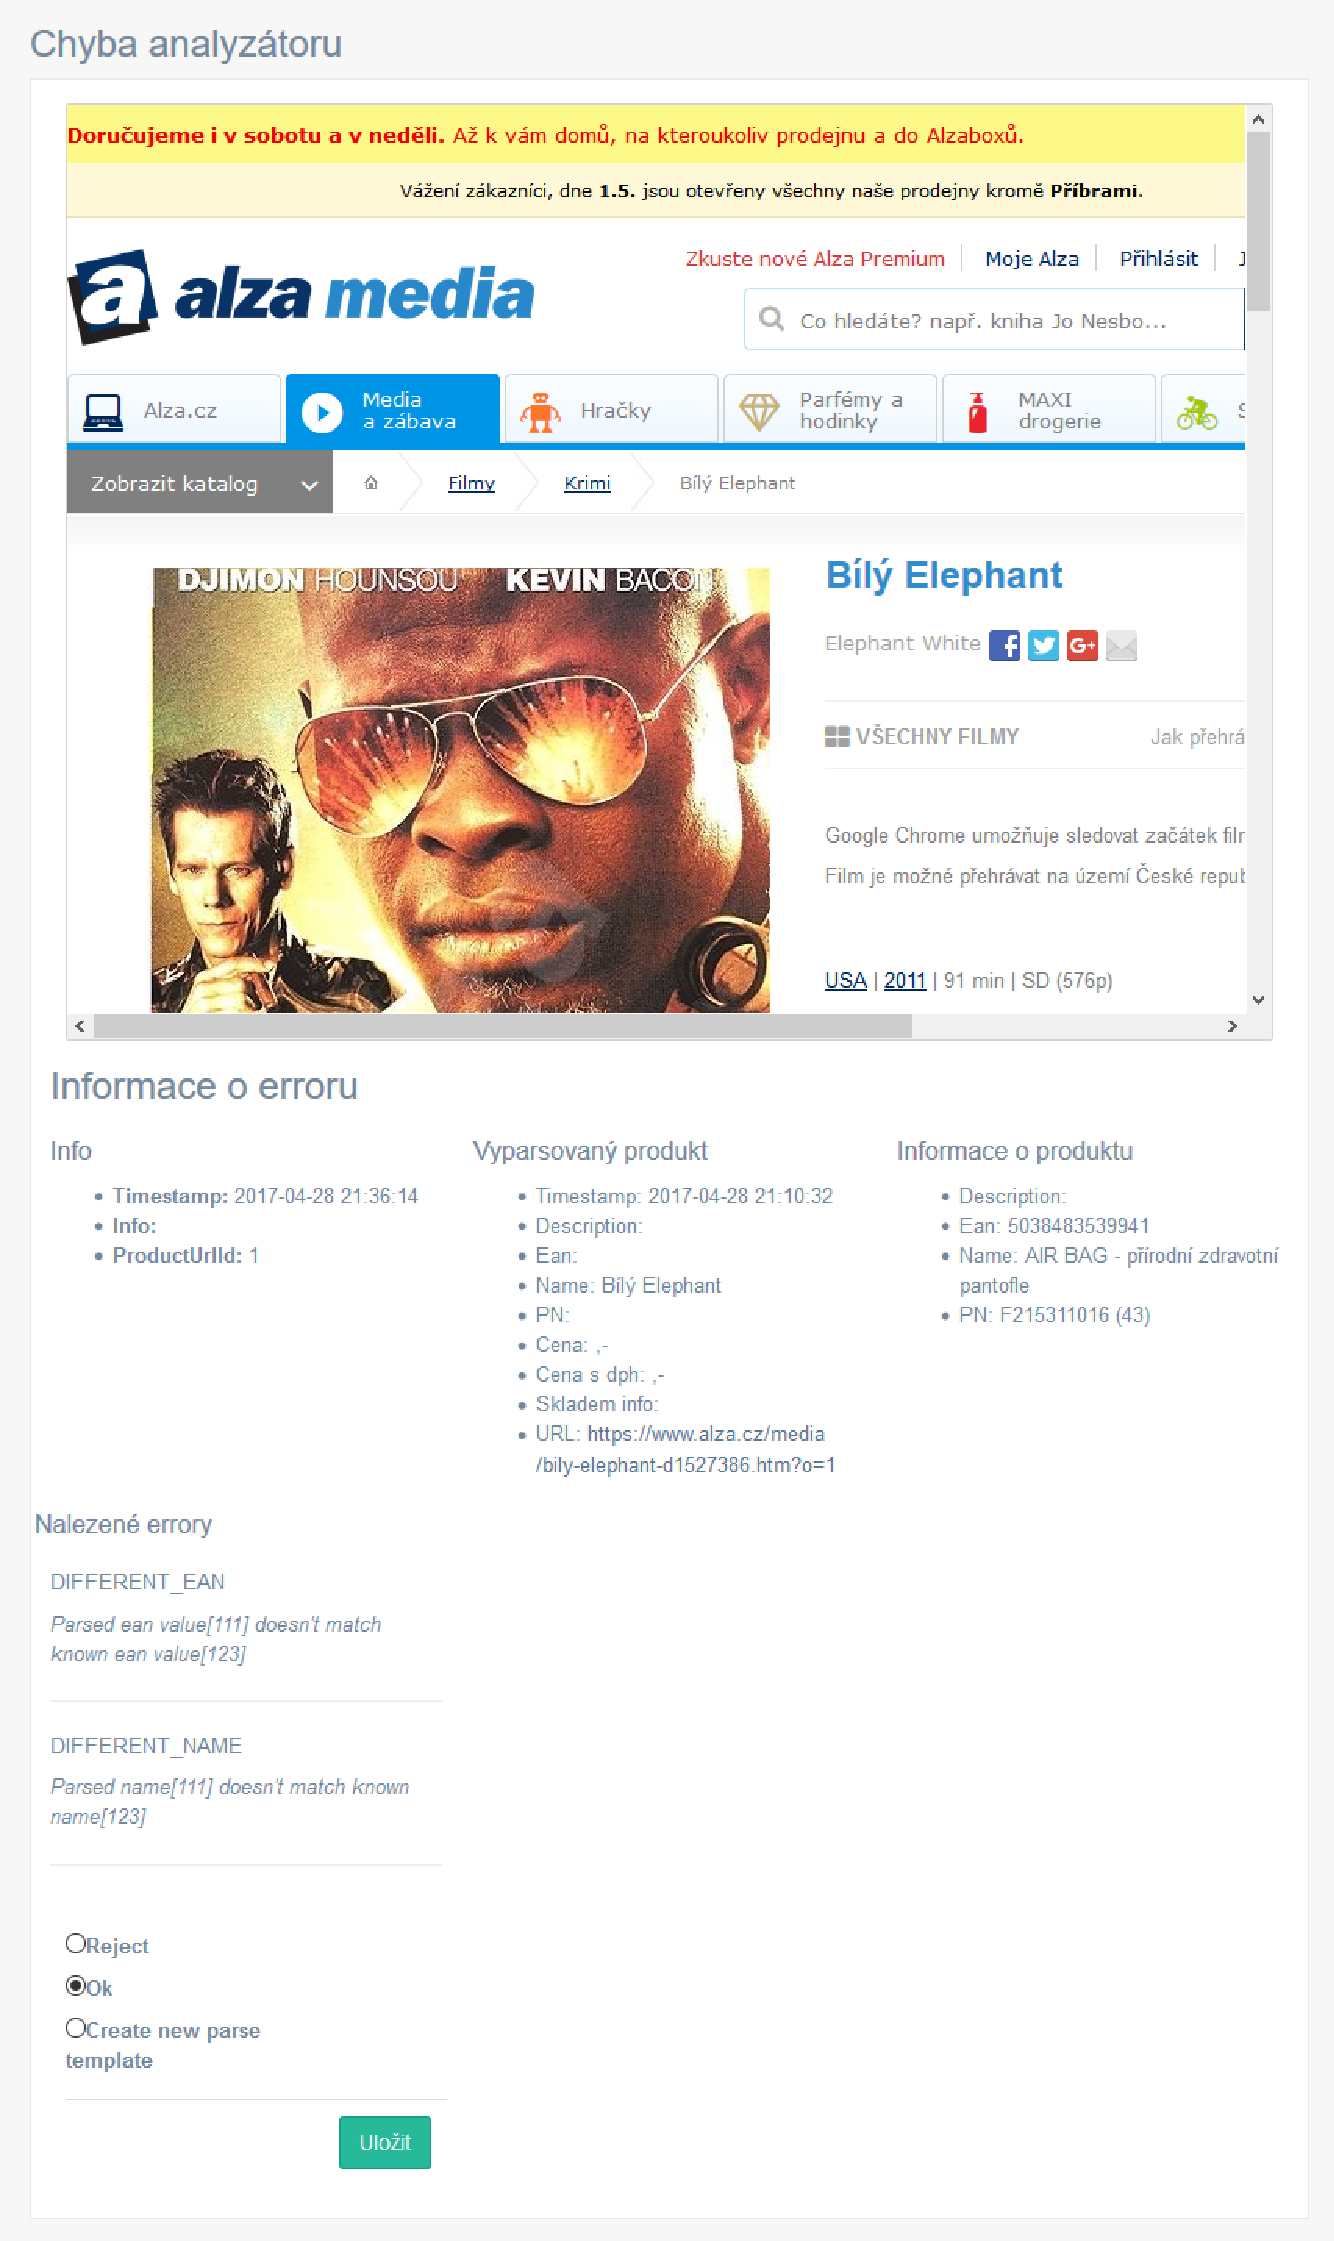
\includegraphics[width=1.0\textwidth]{resources/analyser-err}
	\caption[Webové rozhraní pro vyřešení chyby analyzátoru po provedení vylepšení]{Ukázka webového rozhraní pro vyřešení chyby analyzátoru po provedených vylepšení.}\label{fig:analyser-error}
\end{figure}

\section{Monitorování}
Na virtuální server jsem nasadil službu DataDog \cite{dataDog}, která po jednoduché instalaci umožňuje sledování běžících služeb
a vytížení serveru. Data jsou odesílány přímo do služby DataDog. Webové rozhraní umožňuje sledovat posbírané údaje.
\par
Základní funkcionalita poskytuje pouze informace o využití prostředků a přístup k logům. Službu je však možné rozšířit o velký počet doplňků. Pomocí těch je možné sledovat například výsledek sestavení v Jenkins, ale i obsah a využití RabbitMQ front.


\section{Získání adres obchodů a příslušných detailů produktů}
Vzhledem k malé možnosti využitelnosti implementované části v modulu Finder především z důvodu dlouhých metod, které zajišťují
základní stavební kámen tohoto modulu, jsem se rozhodl modul Finder rozdělit na dvě části.
\par
Část vyhledávající na internetových obchodech adresy detailů popisující diagram aktivit \ref{fig:pdp-diagram} a na část, která samotné obchody vyhledává.
\par
Implementována byla pouze první část, jelikož hledání samotných obchodů lze nahradit manuálním přidání obchodů, na kterých chceme vyhledávat, případně využít některý z veřejných seznamů internetových obchodů v České republice a ty manuálně vložit do databáze.
Jako seznam by bylo možné využít například webovou stránku \href{http://www.i-shopy.cz/}{i-shopy.cz \textit{[cit. 5.5.2017]}}, která indexuje 3091 internetových obchodů.
\par
Modul Finder byl zcela odstraněn a nahrazen modulem novým, nazvaným ProductDetailProvider.
Tento modul zajišťuje hledání detailů produktu, tím je dosaženo na základě šablony pro daný e-shop, která obsahuje 
tyto atributy:
\begin{itemize}
\item formát url vyhledávající produkt na obchodu
\item oddělovač slov v url adrese
\item selektory pro výběr url adres vedoucí na detaily produktu
\end{itemize}
Pro vytvoření požadavku je důležitá existence částečné šablony, která obsahuje informace jak na obchodě vyhledávat.
Po pokusu nalezení adres se vytvoří chyba pro administrátora, aby specifikoval, jak na stránce vyhledávat samotné detaily adres. Webové rozhraní
bylo pro tento proces vytvořeno v rámci týmového projektu.

\begin{figure}\centering
 	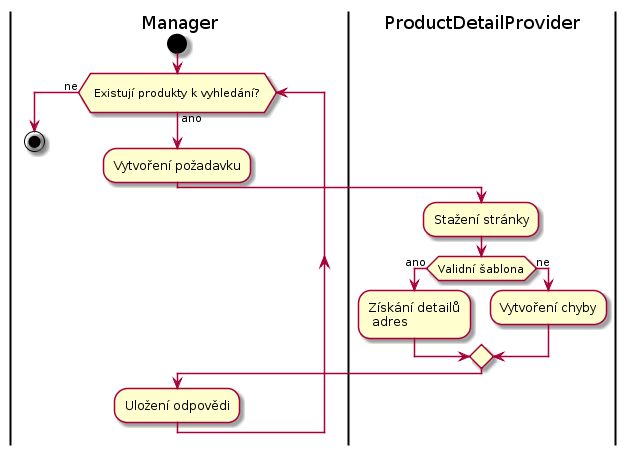
\includegraphics[width=1.0\textwidth]{resources/pdp-activity}
	\caption[Aktivity diagram nalezení adres detailů produktů]{
	Aktivity diagram nalezení adres detailů produktů}\label{fig:pdp-diagram}
\end{figure}

\section{Párování produktu}
Byl navržen proces, který se nejprve pokusí produkt spárovat automaticky, pokud nalezne přímou shodu názvu, EANu nebo modelového čísla.
Pro shodu probíhá hledání podřetězce nalezeného identifikátoru v tom již uloženém. Pokud se hledání nepodaří je vyzkoušeno hledání
podřetězce v opačném směru.
\par
Pokud jsou oba způsoby (pro všechny identifikátory) neúspěšné, jsou provedeny heuristiky hledající pravděpodobné shody. K detekci shody jsou použity algoritmy počítající společná slova a nejdelší společný podřetězec. Z množiny těchto možností je vytvořena chyba, kterou musí zpracovat administrátor.
\par 
Do webového části bylo nutné vytvořit rozhraní, které administrátorovi umožňuje jednoduché přiřazení 
adresy k produktu nebo všechny nabízené možnosti odmítnout.


\section{Detekce neexistující stránky a nenalezeného produktu}
V případě použití interního vyhledávání se stávalo, že pro hledanou hodnotu nebyl nalezen žádný produkt, což bylo zpracování
jako chyba šablony, protože struktura stránky definované šabloně neodpovídala. Podobný případ byl při nalezení adresy detailu, která
ač je obchodem vrácena jako výsledek při hledání, neexistuje. I pro tuto možnost byla vytvořena chyba šablony ve formátu jiného typu.
\par
Nejprve jsem se snažil v případě detekce jiné struktury porovnávat se stránkou, která byla obchodem vrácena při hledání náhodného
řetězce dlouhé délky. Myšlenka byla, že pokud produkt opravdu na obchodu není bude stránka navrácená při hledání s náhodným řetězcem podobná struktura.
\par
Problémem tohoto řešení se ukázala přílišná odlišnost HTML stažených stránek a specifičnost obchodů. Algoritmus fungoval
pouze na malé části obchodů a proto bylo toto řešení zavřeno.
\par
Nakonec jsem zvolil možnost administrátora při řešení chyby zadat řetězec značící neexistenci produktu (popř. neexistující stránky detailu produktu), viz. obrázek \ref{fig:temp-det-err}. Tento řetězec je pro každý obchod specifický a před vytvořením příslušné chyby šablony je nejdříve zkontrolováno, zda
se pouze produkt pouze na obchodě nenachází (popř. stránka neexistuje) a to vyhledání řetězce na stránce. Pokud na stránce řetězec je, pak
se nejedná o chybu šablony.

\begin{figure}\centering
 	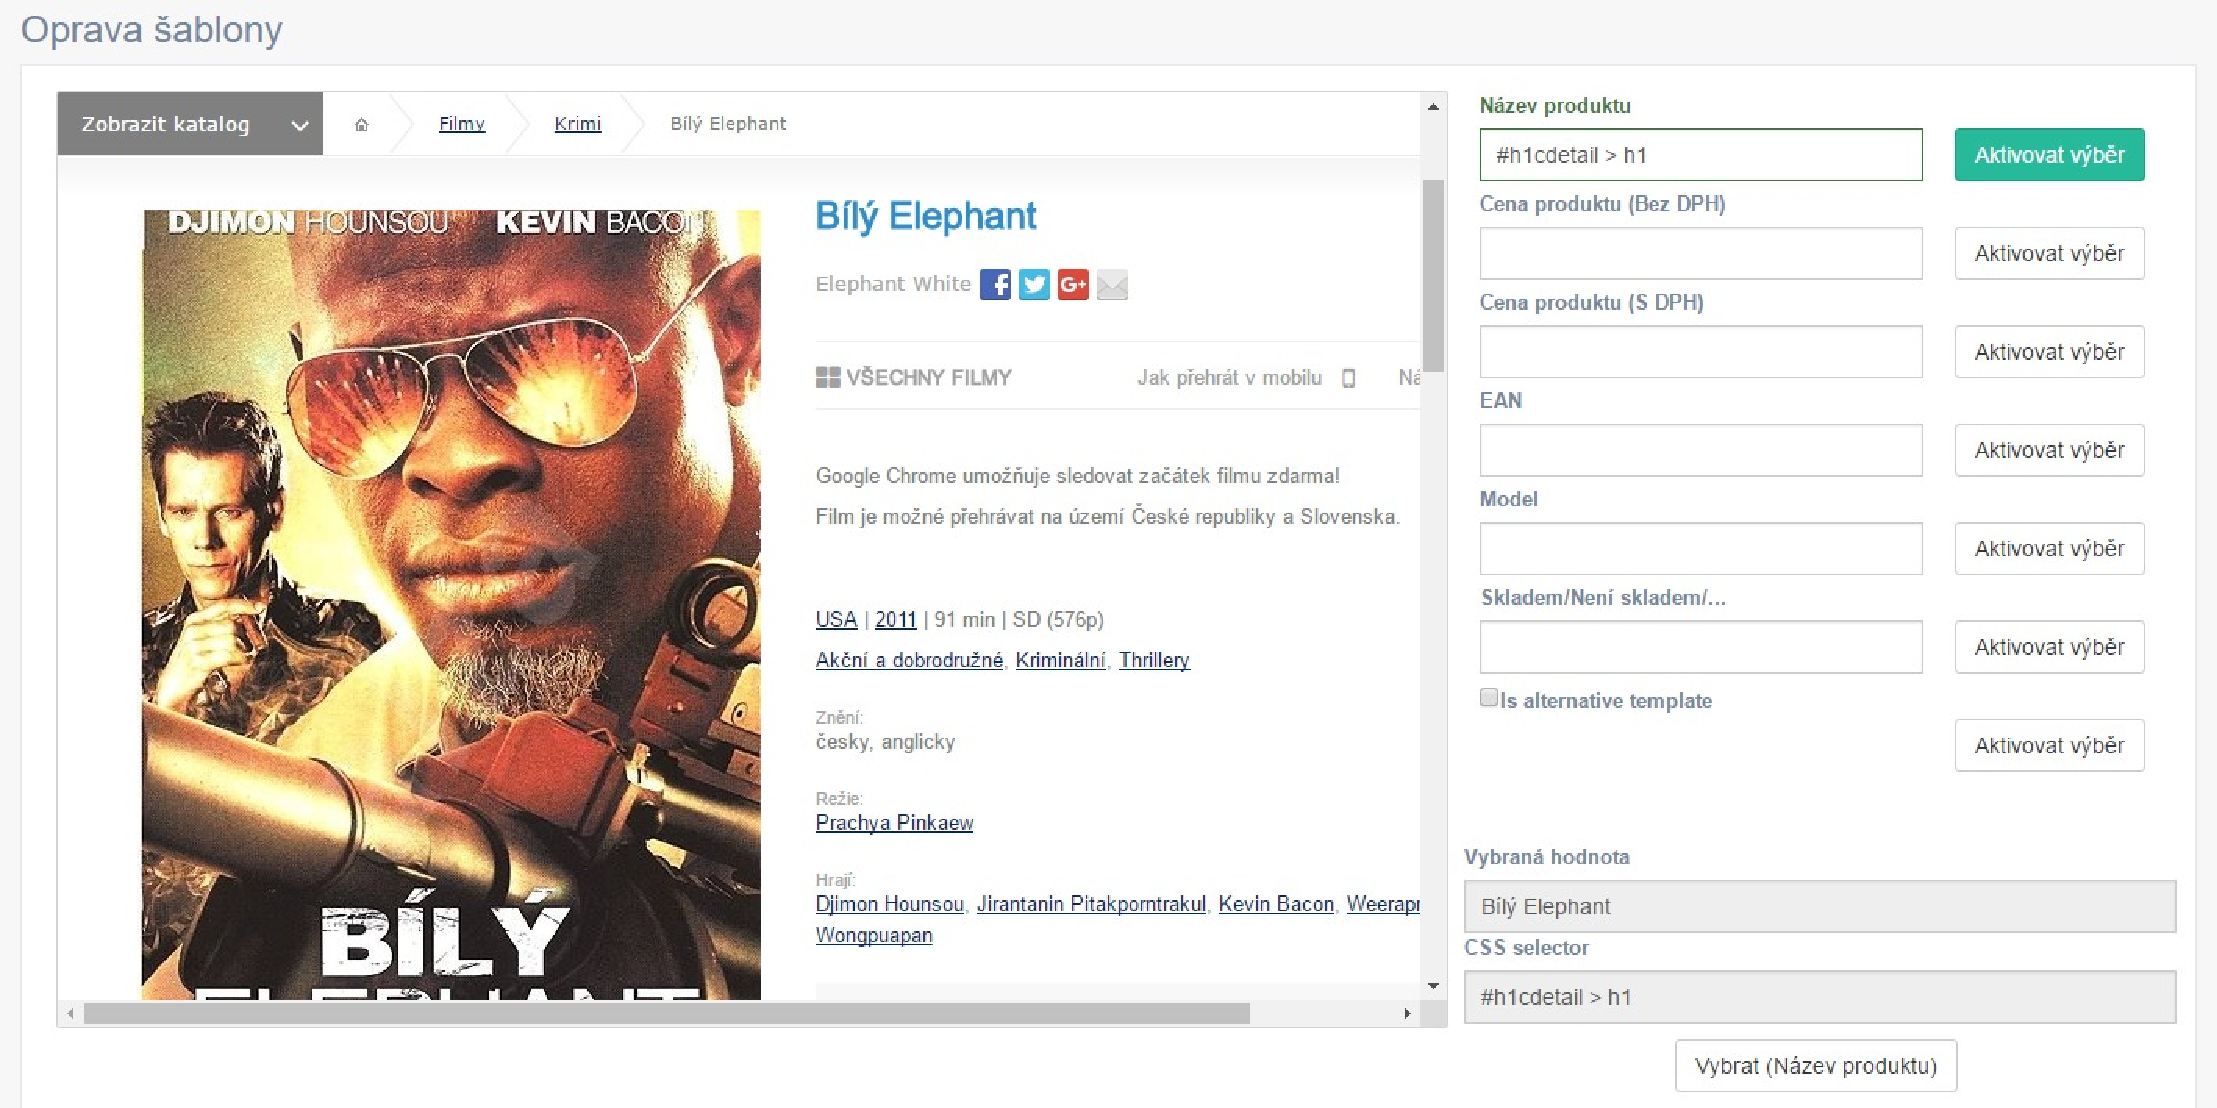
\includegraphics[width=1.0\textwidth]{resources/template-detail-err}
	\caption[Administrátorské rozhraní pro opravu detailu šablony]{Administrátorské rozhraní pro opravu detailu šablony.
	Původnímu řešení neobsahovalo informací v použité url adrese, vyparsované hodnoty a formulář pro chybný řetězec.}\label{fig:temp-det-err}
\end{figure}

\section{Více šablon detailů produktu}
Původní návrh počítal s možností, kdy stránka detailu produktu je ve stejné struktuře napříč celým obchodem.
Tento předpoklad se ukázal jako chybný, například v případě slevy je element obsahující cenu odlišný.
\par
Jiná struktura pak způsobila chybu šablony. Abych problém odstranil implementoval jsem podporu alternativních šablon, které jsou
použity v případě, že hlavní šablona selže. Uložení této šablony jsem zapracoval do rozhraní administrátora, kdy je třeba
vyřešit chybu šablony detailu. Administrátor má možnost původní hlavní šablonu opravit nebo uložit jako alternativní.

\section{Více stejných chyb}
Systém se i po změnách potýkal se stavem, kdy se v administrátorském rozhraní objevilo více chyb šablon nebo analyzátoru.
V původním řešení tento stav nastával tehdy, když neexistovala šablona pro detail nebo vyhledávání na obchodě. 
V případě více požadavků týkajícího se stejného obchodu, vytvoření způsobilo pro každý požadavek chybu.
\par
Chyby lze predikovat a v případě neexistující šablony odeslat pouze jediný požadavek pro ProductProvider.. Ačkoliv jsem pro tento 
stav upravil plánování práce a zároveň přidal kontrolu, která kontroluje zda není takový požadavek již ve frontě, tak
i přesto se stávalo, že administrátor byl zahlcen chybami. Zahlcení v tomto způsobovala šablona, která přestala fungovat.
\par
Tento stav není možné predikovat. Zvolil jsem možnost, kdy je pouze upraveno webové rozhraní a následné uložení opravené chyby.
Úprava webového rozhraní spočívala v zobrazení chyb týkajícího se stejného obchodu v seznamu pouze jednou.
Změna uložení pak způsobí vyřešení i ostatních chyb na obchodu, čímž odpadá nutnost administrátora všechny vyřešit.

\section{Skladem}
V rámci získávání dat u detailu produktu jsem přidal možnost uložit i zda je produkt skladem.
\par
Pro úpravu jsem upravil nejdříve rozhraní pro vytváření šablony a strukturu databáze, aby uchovávala atribut u šablony a výsledku parsování.
Zajistil jsem, aby byl tento atribut zahrnut v rámci komunikace modulu Manager a DataProvider, kde bylo potřeba upravit
správné uložení nových atributů do komunikačních tříd, získání hodnoty při parsování a následné uložení do databáze.

\section{Ostatní}
Při realizaci jsem provedl několik menších změn a oprav. Jedna z nich bylo například nastavení 
připojení do databáze. Původní stav obsahoval konfiguraci  připojení v samostatných \textit{xml} souborech, což znamenalo, že každá nová databázová
třída musela být přidána do všech těchto souborů. 
\par
Tento způsob jsem přepsal, aby nastavení databázových tříd bylo v jednom souboru. Samotné připojení definují
\textit{properties} soubory, které mají následovnou strukturu:

\begin{lstlisting}[language=Java, caption={Nastavení připojení do databáze.}]
hibernate.hikari.dataSource.url
		=jdbc:mysql://localhost:3306/infoweb-db?characterEncoding=UTF-8
hibernate.hikari.dataSource.user=root
hibernate.hikari.dataSource.password=
hibernate.hikari.dataSourceClassName
	=com.mysql.jdbc.jdbc2.optional.MysqlDataSource
database.dialect=org.hibernate.dialect.MySQL5InnoDBDialect
hibernate.hbm2ddl.auto=create-drop
hibernate.hbm2ddl.import_files=sql/importScript.sql
hibernate.hbm2ddl.import_files_sql_extractor
	=org.hibernate.tool.hbm2ddl.MultipleLinesSqlCommandExtractor
\end{lstlisting}

Úprava pak ulehčuje změny v databázových třídách a umožňuje jednoduchou konfiguraci pro více vývojových prostředí jako například testovací, vývojové
a produkční.


\chapter{Zhodnocení provedených vylepšení}
Zde bych se rád věnoval konečné funkcionalitě systému. V návaznosti na výsledný stav popíšu nedostatky objevené v rámci testování, které jsem uskutečnil. Celkové zhodnocení jsem provedl vůči výslednému návrhu a funkcionalitě. Funkcionalitu jsem 
testoval na vzorku produktů popsané v tabulce \ref{product-test} a 20 internetových obchodů.
Pozorování z testování se bude věnovat věnovat v následujících kapitolách.

\begin{table}[h]
\centering
\caption{Tabulka testovaných produktů}
\label{product-test}
\begin{tabular}{@{}lll@{}}
\toprule
\textbf{značka} & \textbf{model}   & \textbf{název}                                                                                                  \\ Scholl          & F215311016 (43)  & \begin{tabular}[c]{@{}l@{}}AIR BAG - přírodní\\ zdravotní pantofle\end{tabular}                                 \\ \midrule
Scholl          & F200781065 (43)  & \begin{tabular}[c]{@{}l@{}}CLOG SUPERCOMFORT\\ bílá\end{tabular}                                                \\ \midrule
Scholl          & 4002448095262    & \begin{tabular}[c]{@{}l@{}}Velvet Smooth wet \& dry \\ - elektrický pilník na chodidla do vody\end{tabular}     \\ \midrule
Beurer          & BEU-FB30         & FB 30 nožní masáž                                                                                               \\ \midrule
Sanitas         & SAN-SEM43        & \begin{tabular}[c]{@{}l@{}}SEM 43 svalový a nervový \\ elektrostimulátor\end{tabular}                           \\ \midrule
Beurer          & BEU-464.15       & \begin{tabular}[c]{@{}l@{}}GL 44 / GL 50 / GL 50 EVO\\ testovací proužky 464.15 (2x25ks)\end{tabular}           \\ \midrule
Beurer          & BEU-IPL10000+    & \begin{tabular}[c]{@{}l@{}}IPL 10000+ Depilace SalonPro \\ System - depilace s dlouhodobým účinkem\end{tabular} \\ \midrule
Salter          & SA1008GSBKXR     & SALTER 1008 GSBKXR                                                                                              \\ \midrule
Homedics        & MIR-8150         & MIR M-8150 - kosmetické zrcadlo                                                                                 \\ \midrule
Philips         & Phil-71768/08/16 & Softpal Battery Olaf White                                                                                      \\ \bottomrule
\end{tabular}
\end{table}


\section{Funkcionalita}
Nejpodstatnější rozdíl při porovnání starého řešení a nového, je samotná funkcionalita, která byla značně rozšířena. Především je možné
využít celý proces hledání informací. Administrátorem stačí zadat přes webové rozhraní obchody na kterých chceme hledat.
Oproti původnímu řešení není nutné definovat adresy detailů přímo vložením do databáze. 
Podpora více šablon rozšiřuje použití na více obchodech.

\section{Kampaň}
Vytvoření kampaně zůstalo stejné jako v původním řešení. Rozdíl je nejvíce markantní v rozhraní pro administrátora, kdy je
možné vyřešit všechny možné chyby, což zajišťuje validní běh kampaně. Výsledek je pak očekávaný výstup, data ze sledovaných
produktů. Uživatel má pak možnost si výstup zobrazit ve webovém rozhraní nebo stáhnout export jako v původním řešení.
\par
Jako nevýhoda a hlavní nedostatek se však ukázal velký důraz na administrátora při řešením prvotních situací, především párování produktů.
\par
Při možném reálném použití systému je pak potřeba zajistit, aby v rámci kampaně byla možnost výběru jaké obchody jsou požadovány sledovat, jelikož
aktuální stav hledá na všech obchodech v systému.


\section{Párování}
Při testování bylo zjištěno, že velké množství obchodů neobsahuje správné nebo přímo odlišné identifikátory produktů. Nejčastější je výskyt pouze jména, které často neodpovídá tomu uloženému.
\par
Párování je nutné na obchodech, které poskytují pouze název, provést ve většině množstvím případů manuálně. Systém se manuální párování snaží ulehčit rozhraním, nicméně i při malém množstvím 
produktů je počet těchto chyb velmi rozsáhlý. 
\par
Proces párování by bylo možné vylepšit, pokud by systém uchovával více identifikátorů. Více uložených jmen by pak zátěž na administrátora mohla s časem klesat, protože použitých jmen napříč obchody by mělo být omezené množství. 
Podpora pro tuto možnost však zcela nebyla zcela implementována, ačkoliv v některých částech byla interní část na tuto možnost již připravena.

\section{Webové rozhraní}\label{ch:web-interface}
Nalezl jsem nedostatky ve webovém rozhraní, kdy jeho funkčnost sloužící k opravám šablony detailu, nebylo na některých obchodech funkční.
Stačilo zadat cestu k elementům manuálně. 
\par
Problém obsahovala i část pro šablonu sloužící k nalezení adres detailů. Pokud bylo použito rozhraní, šablona nebyla ve většině
případů funkční, je proto nutné zadávat cestu k elementu manuálně.

\section{Návrh a testy}
Zásadní refaktoring a změna návrhu komunikace tříd velmi pozměnila interní část. 
Interní část vyhovuje nárokům na formu v původních částech kódu, ale i v případě nové funkcionality. Je složena z přehlednějšího, udržitelnějšího a
lépe rozšiřitelného kódu.
\par
Lepší rozšiřitelnost byla výrazná především při přidávání vylepšení, kdy
tyto změny byly často triviální záležitost a po jejich provedení bylo zachována
původní funkcionalita. Toto dávám za důsledek především lepšího pokrytí
testy a rozdělení tříd do menších celků. Oproti původnímu řešení narostl počet jednotkových
testů ze 170 na 492. Pokrytí demonstruje následující vizualizace.

\begin{figure}[h]\centering
 	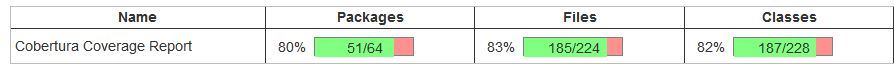
\includegraphics[width=1.0\textwidth]{resources/cobertura-report-new-1}
 	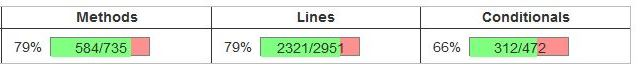
\includegraphics[width=0.7\textwidth]{resources/cobertura-report-new-2}
	\caption[Pokrytí testy po provedených vylepšení]{Pokrytí testy po provedených vylepšení. Získáno pomocí nástroje Cobertura. Vizualizace
	výsledků byla vytvořena při sestavení na Jenkins s příslušným doplňkem.}\label{fig:cober-new}
\end{figure}

Pokrytí vzrostlo zhruba o 20\%. Základní funkcionalita servisních tříd je, až na výjimky testy, pokrytá celá.
Zbylé neotestované třídy jsou především inicializační třídy front a jejich komunikační rozhraní, které je závislé na jiné běžící službě.
\par
I po provedení těchto změn zůstala nemožnost vytvoření více instancí jednotlivých modulů, tedy ProductDetailProvider a DataProvider.
Tato změna je však požadována, až při nárokům na zpracování velkého množství dat. Pro změnu stačí přidat instanční rozhraní jednotlivých modulů, jelikož momentálně jsou spouštěny přímo modulem Manager. Oddělení neovlivní samotnou komunikaci jednotlivých části, nicméně 
vzroste zátěž na nastavení infrastruktury nasazení aplikace na server.

\section{Rozhraní administrátora}
Systém se stal z hlediska pro administrátora uživatelsky přívětivější. Při řešení chyb je rozhraní přehlednější a informace o chybách
obsáhlejší, tím se docílí lepší rozhodování. Dále bylo podstatně zrychleno celkové zpracování. Odpadla nutnost řešit
každý požadavek, ať už se jedná o víc chyb šablon u stejného obchodu či chyb analyzátoru.
\par 
Nevýhodou jsou nedostatky týkající se vytváření šablon, které byly zmíněny v kapitole \ref{ch:web-interface}.

\section{Nemožnost vyhledávání na některých obchodech}
V rámci testování jsem objevil nemožnost vyhledávat na některých obchodech. Jednalo se o dva
menší obchody: \textit{k24.cz} a \textit{elektrocr.cz}. Příčina byla odlišná implementace hledání, kdy nestačilo pouze stáhnout
obsah adresy, která je v příslušném formátu.

\chapter{Závěr}
Vytvořené řešení týmového projektu nevyhovovalo požadavkům na funkcionalitu a možnostem na budoucí rozvoj.
Funkcionalita nebyla splněna především z důvodu nezapojení části, která má za úkol hledat samotné obchody a adresy detailů produktů, které obsahují
hledaná data. Nebyl také vyřešen proces párování produktu k adrese. Návrh některých tříd se ukázal jako nevhodný pro budoucí rozšíření.
\par
V návaznosti na tyto nedostatky bylo navrženo rozsáhlé refaktorování, změna architektury problémových tříd a opravení stávajících
procesů. Bylo potřeba opravit procesy, které nebyly funkční, ztěžovaly práci administrátora nebo byly neefektivní. U funkcionality, kterou měla zajišťovat nezapojená část bylo rozhodnuto o jejím rozdělení, kdy
podpora hledání samotných obchodů byla nahrazena manuálním vložením přes webové rozhraní.
\par
Refaktorování a změna návrhu tříd potvrdila, že se jedná do budoucna o výhodný krok zajišťující lepší udržovatelnost a rozšiřitelnost kódu. Což se ukázalo už při následných změnách, které bylo možné provést v rámci vytvořeného návrhu.
Oprava stávajících procesů pak byla nejvíce viditelná v lepší uživatelské přivětivosti pro administrátora umožňují
případné problémy řešit rychleji a spolehlivěji.
\par
Po implementaci hledání detailu produktu na stránkách obchodů a procesu párování produktů s nalezenými adresami byly
objevené nové nedostatky.
\par
Kritické problémy opravila nová implementace, ale ukázalo se, že i po provedení změn není možné systém použít pro provoz, kde
je požadavek na univerzalitu systému. Systém je po správném nastavení schopný dlouhodobě a automaticky sbírat určitý vzorek dat. Byly však objeveny obchody, kde to není možné. Důvod je především odlišná funkcionalita vyhledávání produktů na sledovaných obchodech, kterou vytvořený systém aktuálně nepodporuje.
\par
Ačkoliv v závěru objevené nedostatky způsobují diskomfort při používání, věřím že přidání funkcionalit navržených v 7. kapitole, umožní plnohodnotné použití výsledného systému.

\bibliographystyle{csn690}



\bibliography{mybibliografy}

\appendix

\chapter{Seznam pojmů}

\section{Web API}
Web Aplication Programming Interface je rozhraní, které na definovaný HTTP dotaz vrátí požadované data. Data jsou standardně vracena ve formátech JSON nebo XML.

\section{Verzovací systém Git}
Git \cite{GIT} je verzovací systém umožňující vytváření a sdílení jednotlivých verzí projektu.
Umožňuje jednoduchý přehled nad rozpracovanými částmi každého vývojáře. Úložiště systému se nazývá repozitář, který obsahuje veškerý kód.
\par
Repozitář existuje v lokálních verzi a zároveň serverové, tedy sdílené. Sdílený repozitář zajišťuje distribuci aktuální verze do lokálních 
repozitářů. Pro lepší správu existují nadstavby nad serverovou částí repozitáře, které umožňují jednoduchou
správu nad kódem a spouštění dalších služeb v závislosti na změnách v kódu.
\par
Základní jednotku tvoří verze, které jsou postupně vytvářeny vývojáři na základě provedených změn.
Verze jsou uchovávány v jednotlivých větvích programu. 
\par
Repozitář je obvykle rozdělen na hlavní a vedlejší větve. Vedlejší větve slouží pro samotný vývoj. 
Hlavní větve tento kód spojují a reprezentují aktuální vývojovou a produkční verzi. Git také obsahuje nástroj pro slučování větví.

\begin{figure}[h]\centering
 	
\includegraphics[width=0.7\textwidth]{resources/branches}
	\caption[Větve v Git repozitáři]{Zobrazení větví v repozitáři, kde \textit{master} je produkční, \textit{develop} vývojová a \textit{topic}
	představuje větev vedlejší}\label{fig:vetev}
\end{figure}

\section{Jednotkové a integrační testy}
Jednotkovými testy se rozumí sada kladných a záporných testů ověřující funkcionalitu jediné třídy. Jednotkové testy
jsou nezávislé na ostatních třídách a testech. \cite{testing} 
\par
Integrační testy pokrývají komunikaci více tříd nebo komunikaci s operačním systémem, hardwarem či rozhraním různých systémů. \cite{testing}
\par
Důvody pro psaní testů jsou například jednodušší nalezení chyby nebo lepší udržovatelnost projektu. V případě neexistujících testů nelze ověřit původní
funkcionalitu při modifikaci aplikace, což může způsobit nutnost nejprve chyby před opravou nalézt.\cite{testing}

\section{Statická analýza kódu}
Statická analýza kódu je analýza softwarového produktu, která běží bez spuštění samotné aplikace. Kontroluje 
pouze kód. Označuje kritické konstrukce vedoucí k chybám nebo nedodržení programátorských konvencí daného
jazyka.
\section{Průběžná integrace}
Průběžnou integrací se rozumí sada nástrojů sloužící k urychlení softwarového vývoje. Základem je průběžné sestavení
a spouštění testů aplikace na základě změn ve sdíleném repozitáři. Lze tak rychle odhalit případné chyby před zařazením 
příslušné verze do produkce.\cite{CI}

\section{Sdílení dat pomocí front}
Sdílení dat pomocí front funguje na principu odesílání zpráv reprezentující objekty. Zprávy jsou po zařazení producentem do fronty odebírány
konzumenty, které je zpracovávají.
Příklad implementace takového systému pak může být RabbitMQ. \cite{rabbitMQ}

\section{JSON}
JSON označuje specifikaci formátu pro výměnu dat\cite{JSON}. Jedná se o formát, který je čitelný nejenom pro lidské oko, ale i pro stroj\cite{JSON},
Zpracování toho formátu je implementováno pro většinu programovacích jazyků\cite{JSON-impl}. Skládá se z párů označující
klíč a hodnotu. Hodnota může být řetězec, číslo nebo pole. Pole pak může uchovávat opět pole, řetězec nebo číslo. \cite{JSON}

\begin{lstlisting}[language=JavaScript, caption={Ukázka formátu JSON}]
{
  "key": [
    1,
    2,
    3
  ],
  "boolean": true,
  "null": null,
  "number": 123,
  "object": {
    "a": "b",
    "c": "d",
    "e": "f"
  },
  "string": "Hello World"
}
\end{lstlisting}

\section{Mock}
V objektově orientovaném programování se Mock objekt používá pro simulování chování konkrétní třídy.\cite{mock}
Při testování je tak možné docílit takových testů, které nejsou závislé na ostatních třídách, kromě té přímo testované.
\par
Testovaná třída obvykle vyžaduje závislost na jiných třídách či rozhraní. Pomocí Mocku je možné chování těchto tříd simulovat.
Mimo nadefinování požadovaného chování, lze také na Mock objektu sledovat jaká na něm byla provedena volání, včetně toho
s jakými parametry. Díky tomu je možné testovat i vnitřní chování testované třídy a ne pouze návratovou hodnotu na základě 
obdrženého vstupu.\cite{mock}

\section{Refaktorování kódu}
Refaktorování v softwarovém vývoji chápeme jako proces restrukturalizace existující kódu, aniž by byla 
pozměněna funkcionalita. Provádí se za účelem dosáhnout průhlednějšího a čitelnějšího kódu, který
se lépe udržuje a rozšiřuje. \cite{refaktoring} Hlavní spouštěcí příčina refaktorování kódu je však existence 
konstrukcí značící špatný návrh aplikace. 

V kontextu této práce jsou důležité především následující konstrukce značící možné problémy \cite{refaktoring}:  
\begin{itemize}
\item Dlouhá metoda
\item Velká třída
\item Dlouhý seznam parametrů
\item Složité struktury podmínek
\end{itemize}

\chapter{Seznam použitých zkratek}
% \printglossaries
\begin{description}
	\item[EAN] European Article Number
	\item[XML] Extensible markup language
	\item[HTML] Hypertext Markup Language
	\item[CSS] Cascading style sheets
	\item[JSON] JavaScript Object Notation
	\item[HTTP] Hypertext Transfer Protocol
	\item[DAO] Data Access Object
	\item[URL] Uniform Resource Locator

\end{description}

% % % % % % % % % % % % % % % % % % % % % % % % % % % % 
% % Tuto kapitolu z výsledné práce ODSTRAŇTE.
% % % % % % % % % % % % % % % % % % % % % % % % % % % % 
% 
% \chapter{Návod k~použití této šablony}
% 
% Tento dokument slouží jako základ pro napsání závěrečné práce na Fakultě informačních technologií ČVUT v~Praze.
% 
% \section{Výběr základu}
% 
% Vyberte si šablonu podle druhu práce (bakalářská, diplomová), jazyka (čeština, angličtina) a kódování (ASCII, \mbox{UTF-8}, \mbox{ISO-8859-2} neboli latin2 a nebo \mbox{Windows-1250}). 
% 
% V~české variantě naleznete šablony v~souborech pojmenovaných ve formátu práce\_kódování.tex. Typ může být:
% \begin{description}
% 	\item[BP] bakalářská práce,
% 	\item[DP] diplomová (magisterská) práce.
% \end{description}
% Kódování, ve kterém chcete psát, může být:
% \begin{description}
% 	\item[UTF-8] kódování Unicode,
% 	\item[ISO-8859-2] latin2,
% 	\item[Windows-1250] znaková sada 1250 Windows.
% \end{description}
% V~případě nejistoty ohledně kódování doporučujeme následující postup:
% \begin{enumerate}
% 	\item Otevřete šablony pro kódování UTF-8 v~editoru prostého textu, který chcete pro psaní práce použít -- pokud můžete texty s~diakritikou normálně přečíst, použijte tuto šablonu.
% 	\item V~opačném případě postupujte dále podle toho, jaký operační systém používáte:
% 	\begin{itemize}
% 		\item v~případě Windows použijte šablonu pro kódování \mbox{Windows-1250},
% 		\item jinak zkuste použít šablonu pro kódování \mbox{ISO-8859-2}.
% 	\end{itemize}
% \end{enumerate}
% 
% 
% V~anglické variantě jsou šablony pojmenované podle typu práce, možnosti jsou:
% \begin{description}
% 	\item[bachelors] bakalářská práce,
% 	\item[masters] diplomová (magisterská) práce.
% \end{description}
% 
% \section{Použití šablony}
% 
% Šablona je určena pro zpracování systémem \LaTeXe{}. Text je možné psát v~textovém editoru jako prostý text, lze však také využít specializovaný editor pro \LaTeX{}, např. Kile.
% 
% Pro získání tisknutelného výstupu z~takto vytvořeného souboru použijte příkaz \verb|pdflatex|, kterému předáte cestu k~souboru jako parametr. Vhodný editor pro \LaTeX{} toto udělá za Vás. \verb|pdfcslatex| ani \verb|cslatex| \emph{nebudou} s~těmito šablonami fungovat.
% 
% Více informací o~použití systému \LaTeX{} najdete např. v~\cite{wikilatex}.
% 
% \subsection{Typografie}
% 
% Při psaní dodržujte typografické konvence zvoleného jazyka. České \uv{uvozovky} zapisujte použitím příkazu \verb|\uv|, kterému v~parametru předáte text, jenž má být v~uvozovkách. Anglické otevírací uvozovky se v~\LaTeX{}u zadávají jako dva zpětné apostrofy, uzavírací uvozovky jako dva apostrofy. Často chybně uváděný symbol "{} (palce) nemá s~uvozovkami nic společného.
% 
% Dále je třeba zabránit zalomení řádky mezi některými slovy, v~češtině např. za jednopísmennými předložkami a spojkami (vyjma \uv{a}). To docílíte vložením pružné nezalomitelné mezery -- znakem \texttt{\textasciitilde}. V~tomto případě to není třeba dělat ručně, lze použít program \verb|vlna|.
% 
% Více o~typografii viz \cite{kobltypo}.
% 
% \subsection{Obrázky}
% 
% Pro umožnění vkládání obrázků je vhodné použít balíček \verb|graphicx|, samotné vložení se provede příkazem \verb|\includegraphics|. Takto je možné vkládat obrázky ve formátu PDF, PNG a JPEG jestliže používáte pdf\LaTeX{} nebo ve formátu EPS jestliže používáte \LaTeX{}. Doporučujeme preferovat vektorové obrázky před rastrovými (vyjma fotografií).
% 
% \subsubsection{Získání vhodného formátu}
% 
% Pro získání vektorových formátů PDF nebo EPS z~jiných lze použít některý z~vektorových grafických editorů. Pro převod rastrového obrázku na vektorový lze použít rasterizaci, kterou mnohé editory zvládají (např. Inkscape). Pro konverze lze použít též nástroje pro dávkové zpracování běžně dodávané s~\LaTeX{}em, např. \verb|epstopdf|.
% 
% \subsubsection{Plovoucí prostředí}
% 
% Příkazem \verb|\includegraphics| lze obrázky vkládat přímo, doporučujeme však použít plovoucí prostředí, konkrétně \verb|figure|. Například obrázek \ref{fig:float} byl vložen tímto způsobem. Vůbec přitom nevadí, když je obrázek umístěn jinde, než bylo původně zamýšleno -- je tomu tak hlavně kvůli dodržení typografických konvencí. Namísto vynucování konkrétní pozice obrázku doporučujeme používat odkazování z~textu (dvojice příkazů \verb|\label| a \verb|\ref|).
% 
% \begin{figure}\centering
% 	
\includegraphics[width=0.5\textwidth, angle=30]{cvut-logo-bw}
% 	\caption[Příklad obrázku]{Ukázkový obrázek v~plovoucím prostředí}\label{fig:float}
% \end{figure}
% 
% \subsubsection{Verze obrázků}
% 
% % Gnuplot BW i barevně
% Může se hodit mít více verzí stejného obrázku, např. pro barevný či černobílý tisk a nebo pro prezentaci. S~pomocí některých nástrojů na generování grafiky je to snadné.
% 
% Máte-li například graf vytvořený v programu Gnuplot, můžete jeho černobílou variantu (viz obr. \ref{fig:gnuplot-bw}) vytvořit parametrem \verb|monochrome dashed| příkazu \verb|set term|. Barevnou variantu (viz obr. \ref{fig:gnuplot-col}) vhodnou na prezentace lze vytvořit parametrem \verb|colour solid|.
% 
% \begin{figure}\centering
% 	\includegraphics{gnuplot-bw}
% 	\caption{Černobílá varianta obrázku generovaného programem Gnuplot}\label{fig:gnuplot-bw}
% \end{figure}
% 
% \begin{figure}\centering
% 	\includegraphics{gnuplot-col}
% 	\caption{Barevná varianta obrázku generovaného programem Gnuplot}\label{fig:gnuplot-col}
% \end{figure}
% 
% 
% \subsection{Tabulky}
% 
% Tabulky lze zadávat různě, např. v~prostředí \verb|tabular|, avšak pro jejich vkládání platí to samé, co pro obrázky -- použijte plovoucí prostředí, v~tomto případě \verb|table|. Například tabulka \ref{tab:matematika} byla vložena tímto způsobem.
% 
% \begin{table}\centering
% 	\caption[Příklad tabulky]{Zadávání matematiky}\label{tab:matematika}
% 	\begin{tabular}{|l|l|c|c|}\hline
% 		Typ		& Prostředí		& \LaTeX{}ovská zkratka	& \TeX{}ovská zkratka	\tabularnewline \hline \hline
% 		Text		& \verb|math|		& \verb|\(...\)|	& \verb|$...$|		\tabularnewline \hline
% 		Displayed	& \verb|displaymath|	& \verb|\[...\]|	& \verb|$$...$$|	\tabularnewline \hline
% 	\end{tabular}
% \end{table}
% 
% % % % % % % % % % % % % % % % % % % % % % % % % % % % 

\chapter{Obsah přiloženého CD}

%upravte podle skutecnosti

\begin{figure}
	\dirtree{%
		.1 readme.txt\DTcomment{stručný popis obsahu CD}.
		.1 build\DTcomment{adresář se sestavenými verzemi systému}.
		.2 backend\DTcomment{adresář obsahující sestavenou interní část}.
		.2 backend-old\DTcomment{adresář obsahující ses. interní část původního řešení}.
		.1 docs\DTcomment{dokumentace systémuom}.
		.2 backend\DTcomment{dokumentace interní částí}.
		.2 frontend\DTcomment{dokumentace webového rozhraní}.
		.1 src\DTcomment{zdrojové kódy implementace}.
		.2 backend\DTcomment{zdrojové kódy interní částí}.
		.2 backend\DTcomment{zdrojové kódy interní částí původního řešení}.
		.2 frontend\DTcomment{zdrojové kódy webového rozhraní}.
		.2 frontend\DTcomment{zdrojové kódy webového rozhraní původního řešení}.
		.1 text\DTcomment{zdrojová forma práce ve formátu \LaTeX{}}.
		.2 thesis.pdf\DTcomment{text práce ve formátu PDF}.
	}
\end{figure}

\end{document}
